\documentclass[10pt,a4paper]{article}


\usepackage[margin=3cm]{geometry}
\usepackage[UKenglish]{babel}
\usepackage{enumitem}
\usepackage{calc}
\usepackage{fancyhdr}
\usepackage{graphicx}
\usepackage{multirow}
\usepackage[table]{xcolor}
\usepackage{float}
\usepackage{longtable}
\usepackage{parskip}
\usepackage{soul}
\usepackage[small,compact]{titlesec}
\usepackage[justification=centering]{caption}

\definecolor{reqColor}{RGB}{80,80,120}
\definecolor{titleColor}{RGB}{138,201,242}
\pagestyle{fancy}
\lhead{T Davies, A Fahie, A Fairbairn, A Free, J Mansfield, R Tucker, M 
Walker}
\chead{}
\rhead{GPIG-C}
\cfoot{\vspace{-0.6cm} \thepage}

\setlist{nolistsep} % Reduces lots of white space around lists

\renewcommand{\headrulewidth}{0.4pt} % Add rules below header
\renewcommand*{\thefootnote}{\fnsymbol{footnote}}

\newcommand{\conreq}[1]{\textcolor{reqColor}{\textbf{CR.#1}}}
\newcommand{\fr}[1]{\textcolor{reqColor}{\textbf{FR.#1}}}
\newcommand{\frit}[1]{\textit{FR.#1}}
\newcommand{\nfr}[1]{\textcolor{reqColor}{\textbf{NFR.#1}}}
\newcommand{\nfrit}[1]{\textit{NFR.#1}}

\begin{document}

\begin{center}
{\Large GPIG-C Interim Report}

%Word count: @WORD_COUNT@
\unskip
\footnote{\textit{Using TeXCount, excluding\ldots}} %%Really?

Friday, 14th February 2014
\end{center}

\vspace{0.3cm}
\rule{\textwidth}{0.4pt}
\section{Glossary}
\label{sec:glossary}

\begin{description}[leftmargin=!,labelwidth=\widthof{\bfseries Data output clientxx},itemsep=0.1cm]
	\item[The HUMS/System] The health and usage monitoring system being developed
	\item[(HUMS) Instance] A particular deployment of the System
	\vspace{0.2cm}
	\item[Customer] Thales, the organisation that has commissioned the System
	\item[Consumer] An organisation that makes use of the System
	\item[Consumer System] The system that a Consumer wishes to monitor
	\item[(End) User] An individual that uses the System within a Consumer organisation
	\vspace{0.2cm}
	\item[Client] Computer hardware or software that interfaces with an Instance
	\item[Input Interface] The interface through which data is supplied to an Instance
	\item[Data Emitter] A Client that provides data to an Instance through the Input Interface
	\item[Output Interface] The interfaces through which reports and notifications are dispatched
	\item[Data Output Client] A Client that receives data from an Instance through an Output Interface
	\vspace{0.2cm}
	\item[Analysis] The processing of data performed by the System
	\item[Event] A point of interest identified by Analysis
	\item[Notification] A message dispatched by the System when an Event is fired
	\item[Report] A message produced by the System by request of a User
	\vspace{0.2cm}
	\item[Sensor] A source of data to be monitored by the System
	\item[System ID] A unique identifier given to each Client of a particular Instance
\end{description}

\section{Introduction}
\label{sec:introduction}



\section{Requirements Refinement}
\label{sec:requirements}
After feedback from the initial report the original requirements have been 
altered and, where possible, refined.

\subsection{Functional Requirements}
\label{sec:requirements-functional}
Below, the existing functional requirements are refined, based on customer 
feedback and design decisions made in the previous report.

\frit{1} is refined to specify how data emitters will send data to the system, 
and the type of data required. 
\frit{2} required data to be timestamped, but didn't specify how these 
timestamps were to be produced, \frit{2.1} and \frit{2.2} assign this
responsibility to the data emitter and consumer system, mandating when 
timestamps should be created.

\frit{3} is refined by specifying how the data is to be stored, allowing the end 
user to choose the technology of their choice, meaning the database can be 
changed without needing to alter other modules, making it easy to 
port the HUMS across domains.
\frit{4} was modified such that the previous requirements \frit{4}, \frit{6}, 
\frit{9}, and \frit{10} can all be expressed as refinements, with the 
configuration files containing all end user settings. The new \frit{5} and \frit{6} 
enforce the  functionality the HUMS must provide as a result of the data 
in the configuration file.

\frit{7}, previously \frit{12}, is refined to define how data will be analysed for 
events. It identifies that there must be an API allowing analysis engines, 
either created by the Consumer or included with the HUMS, to extract stored 
data and produce events. 

\frit{9} to \frit{12} do not appear in the previous report, and were discovered 
to be necessary following feedback from the customer regarding the ability 
of the system to allow for explicit feedback: the output of analysis must be able to affect the monitored system. 
It was felt that our architecture did not make it clear whether this was 
possible or not, therefore these requirements were added as clarification.
\begin{description}
	%%FR1
  	\item[\fr{1}]  Data emitters shall be able to push correctly structured 
data 	to the HUMS.
	\begin{description}[leftmargin=1.3cm]
		 \item[\fr{1.1}] The HUMS shall provide an API for data input.
		\begin{description}
			  \item[\fr{1.1.1}] The data input API shall require an ID	
			for the consumer system.
 			 \item[\fr{1.1.2}] The data input API shall require data to be
 		 	timestamped.
 			 \item[\fr{1.1.3}] The data input API shall allow data emitters
 		 	to send sensor IDs and their values to the HUMS, 		
			which will then be made available to an analysis engine.
		\end{description}
 		 \item[\fr{1.2}] A data emitter, extracting data from the given 	
	test application, shall be provided.
	\end{description}
	%%FR2
	\item[\fr{2}]  The HUMS shall allocate a timestamp to new data.
	\begin{description}
	 	 \item[\fr{2.1}]Data input clients shall timestamp data before
 		sending it to the HUMS.
 		 \item[\fr{2.2}] Timestamps shall be collected when data is sent 	
		to storage.
	\end{description}
	%%FR3
	 \item[\fr{3}] The HUMS shall store correctly structured data.
	 \begin{description}
	 	\item[\fr{3.1}] The end user shall integrate their chosen database 
			technology with the HUMS.
	 	\item[\fr{3.2}] The HUMS shall use a database abstraction layer, 
			allowing the database component to be easily changed 
                                according to needs.
	  \end{description}
	%%FR4
	 \item[\fr{4}] The HUMS shall store end user system configuration 
			files.
	 \begin{description}
	  	\item[\fr{4.1}] The HUMS shall allow authorised users to modify
 		configuration files. 
		 \item[\fr{4.2}] The HUMS shall allow the consumer to define a 	
			low storage threshold.
		  \item[\fr{4.3}] The HUMS shall allow the consumer to set an 
			expiry time on data.
		  \item[\fr{4.4}] The HUMS shall allow the user to define that, 
			upon reaching their defined data storage quota, new data is 
			no longer added.
		 \item[\fr{4.5}] The HUMS shall allow the user to define that, 
			upon reaching their defined data storage limit, old data is 
			deleted to make room for new data.
	\end{description}
	%%FR5
	 \item[\fr{5}] The HUMS shall send a notification when the consumer's 
		low storage threshold is reached.
	  \item[\fr{6}] The HUMS must store no more data records than the 	
		consumer's defined storage quota.
	\item[\fr{7}]Events shall be triggered in response to data matching a pattern 
	specified by the consumer.
		  \begin{description}
			 \item[\fr{7.1}]  The HUMS shall allow the user to specify 	
			what data patterns will produce events.
			 \item[\fr{7.2}] The HUMS shall allow the user to define their
 			own events.
 			\item[\fr{7.3}] The HUMS shall provide an API, 			
			allowing analysis engines to extract stored data.
			\item[\fr{7.4}] Events shall be created by analysis engines.
 			\item[\fr{7.5}] The HUMS shall provide a simple analysis 	
			engine in the form of a rules engine.
	\end{description}
	
	\item[\fr{8}]After the sending of a notification for an event of a particular 
		type, no more notifications for an event of that type will be 	
		sent during the cool down period.
	\item[\fr{9}]The HUMS shall dispatch an event when a specified data 
		pattern is detected.
	\item[\fr{10}] The HUMS must interface with reports engines, allowing 
		them to pull reports.
	\item[\fr{11}] The system shall allow for notifications to change the way 
		in which data is sensed.
	 \item[\fr{12}] The system shall allow notifications to be sent back to 
		the system being monitored.
\end{description}

\subsection{Non-Functional Requirements}
Non-functional requirements remain similar, however \nfrit{14} has been 
added in order to clarify that data can be sent and stored in any format, 
enforcing that the consumer's system will not have to conform to a format
dictated by the HUMS. \nfrit{6} has been refined to more concretely detail the
testing strategies to be used when validating that requirements have been met.
It is also recognised that \nfrit{5} and \nfrit{11} are requirements 
specific to the prototype as the functional requirements mandate that the 
datastore be changeable, meaning, in the general case, requirements 
about the abilities of the datastore are not verifiable.
\begin{description}
	\item[\nfr{1}] The HUMS shall receive hardware changes without loss 
	of previously stored data.
	\item[\nfr{2}]  Users shall be provided with documentation detailing 
	how 	to use the HUMS.
	\item[\nfr{3}] The HUMS must be accessible to end users in multiple 	
	geographic locations.
	\item[\nfr{4}]  The HUMS shall only accept data from an input client 	
	providing valid credentials. 
	\item[\nfr{5}] The HUMS shall store data according to the relevant 	
	industry security standards. 
	\item[\nfr{6}]  The HUMS shall be tested to ensure all requirements are 
	met before deployment.
	\begin{description}
	\item[\nfr{6.1}]  The HUMS shall be tested using unit testing.
	\item[\nfr{6.2}]  The HUMS shall be tested using integration testing.
	\item[\nfr{6.3}]  The HUMS shall be tested using system testing.
	\item[\nfr{6.4}]  The HUMS shall be tested using inspection.
	\item[\nfr{6.5}]  The HUMS shall be tested using acceptance testing.
	\end{description}
	\item[\nfr{7}] The customer will complete acceptance testing before the 
	system is deployed.
	\item[\nfr{8}] The system must be able to support at least 5 output 
	clients per HUMS instance. 
	\item[\nfr{9}] The system must be available for no less than 99.9\% of 
	each month.
	\item[\nfr{10}]  Data must be backed up within 24 hours of having been 
	made available to the system.
	 \item[\nfr{11}] Timestamps applied by the system must be accurate to 
	within 5ms of UTC.
	\item[\nfr{12}]  The system shall dispatch notifications within 5ms of an 
	event being triggered.
	\item[\nfr{13}] The system shall support storing data without requiring 
	specific schemata.
\end{description}

\subsection{Constraint Requirements}
The constraint requirements have been modified to include other external dependencies identified due to the design decisions made throughout the previous phase of the project, including dependancies on technology choices. Previous constraints restricting the schema of data stored in the HUMS have been removed, as feedback suggested that this should not be the responsibility of the consumer.
\begin{description}
	\item[\conreq{1}]  The system will be presented with valid credentials 	by the consumers data emitters.
	\item[\conreq{2}]  Valid output clients for the system will be specified 		by the consumer.	
	\item[\conreq{3}]  The hardware that the system runs on will be 			supported by the JVM.
	\item[\conreq{4}]  The system will have access to the network to which 	the data sources are connected.
	\item[\conreq{5}]  The customer will provide two test applications 		across the course of the project.
	\item[\conreq{6}]  The customer will receive an interim report detailing 	project progress no later 14/02/2014.
	\item[\conreq{7}] The customer will receive a final report detailing the 	proposed system no later than 28/05/2014. 
	\item[\conreq{8}]  The customer will be presented with a system 		prototype on 30/05/2014.
	\item[\conreq{9}] The development team will be comprised of seven 		software engineers.
\end{description}


\section{System Architecture}
\label{sec:architecture}

\subsection{Quality Attributes}
\label{sec:architecture-quality}

Quality attributes are defined in order to ensure the architectural decisions 
made when creating the system architecture not only provide the required 
functionality, but also produce a system meeting the expectations of all 
stakeholders. For example the system may be expected to meet certain 
security standards or availability levels. Explicitly defining these quality 
attributes before concretely designing a system allows for the correct 
tactics and patterns to be adopted in order to maximise the utility of important 
qualities. When examining the HUMS non-functional requirements the 
following system quality attributes were identified:
	\begin{center}
	\textit{Flexibility, Performance, Modifiability, Security, 
Testability, Usability}
	\end{center}
For the prototype implementation, at this stage, usability and security 
have not been heavily considered, however in the real system they 
would be of high importance. Security is a key aspect of any nontrivial HUMS, 
as data being monitored must be both secret and safe. It must be impossible 
for an unauthorised user to either insert or remove data from the system, and 
so all data would need to be stored according to relevant security standards 
(e.g., encryption and password protection for personal data covered by the 
Data Protection Act). Additionally, data in transit between emitters and the data 
input API must be protected, which can be achieved using a symmetric-key 
encryption system, which is well supported by many programming languages. 
Determining who has the rights to access which data would fall under the 
purview of an individual customer, who would manage access rights using the 
configuration front-end of our system.

Flexibility is important to the HUMS as it is to be used across multiple 
domains, meaning it cannot be too specific. Following a plugin 
architecture means the system can remain general and flexible however 
can include domain specific elements, such as analysis engines, 
creating a software product line where the core of the HUMS can be 
shared across all domains.

Modifiability is also an important quality of the HUMS and, though not 
measurable, lack of modifiability can increase the cost and time taken to 
complete the project. The HUMS will initially be built to tackle a single 
domain (software), however will in the future be required to work on embedded 
systems, mechanical systems, electrical systems and even people. In 
order to ensure these changes are as efficient as possible the initial system 
must be modifiable. Tactics that can be used to increase the modifiability 
of the system include using small modules within the system, decreasing the 
coupling between those modules and increasing the cohesion. In order 
to achieve low coupling  the HUMS uses interfaces between modules and 
restricts dependencies, such that the majority of modules can be 
swapped out without large changes to the overall system.

The performance of a system is normally measured by its latency and 
throughput. The HUMS is required to dispatch notifications through the 
notification generator after events have been triggered by the analysis 
controller, with a latency less than 5ms. The system is also required to be
able to support multiple data output clients. Tactics such as reducing
overhead though careful use of data structures and prioritising events can
help reduce latency, at least for the most important events, defined by the
end user. It may also be possible to add concurrency, such that multiple
notification threads are used when demand for notifications and reports are
high, reducing the bottleneck created at the notification generator.

In in order to ensure the HUMS is testable we followed the test driven 
development (TDD) methodology where possible, writing and planning the tests 
before writing the code, so passing tests means code performs the 
expected functionality. In addition to this we also defined how 
each requirement of the system would be tested and created a 
comprehensive test plan, detailing integration, system, unit and 
acceptance testing.

\section{System Views}
\label{sec:architecture-views}

When designing the HUMS we identified four different views of the
system which must be documented, taking inspiration from the
Hofmeister\cite{hof1999} approach to software architecture:

\begin{description}
  \item[Module View] The required software modules and relationships
    between them at a high level.

  \item[Behavioural View] The flow of data and dynamic actions within
    the system.

  \item[Execution View] How modules are geographically positioned.

  \item[Conceptual View] Class diagrams, showing a concrete
    implementation of the functionality.
\end{description}

\subsection{Module View}
\label{sec:architecture-moduleview}

Having determined the quality attributes of the HUMS and the tactics
which can be employed in order to achieve a high utility of these
qualities, a conceptual view can be formed. The conceptual diagram
shown in figure \ref{fig:ComponentDiagram} depicts the modules of the
HUMS and the interactions between these modules at a high level.

%%TODO this diagram doesn't have a key

\begin{figure}[!ht]
  \centering
  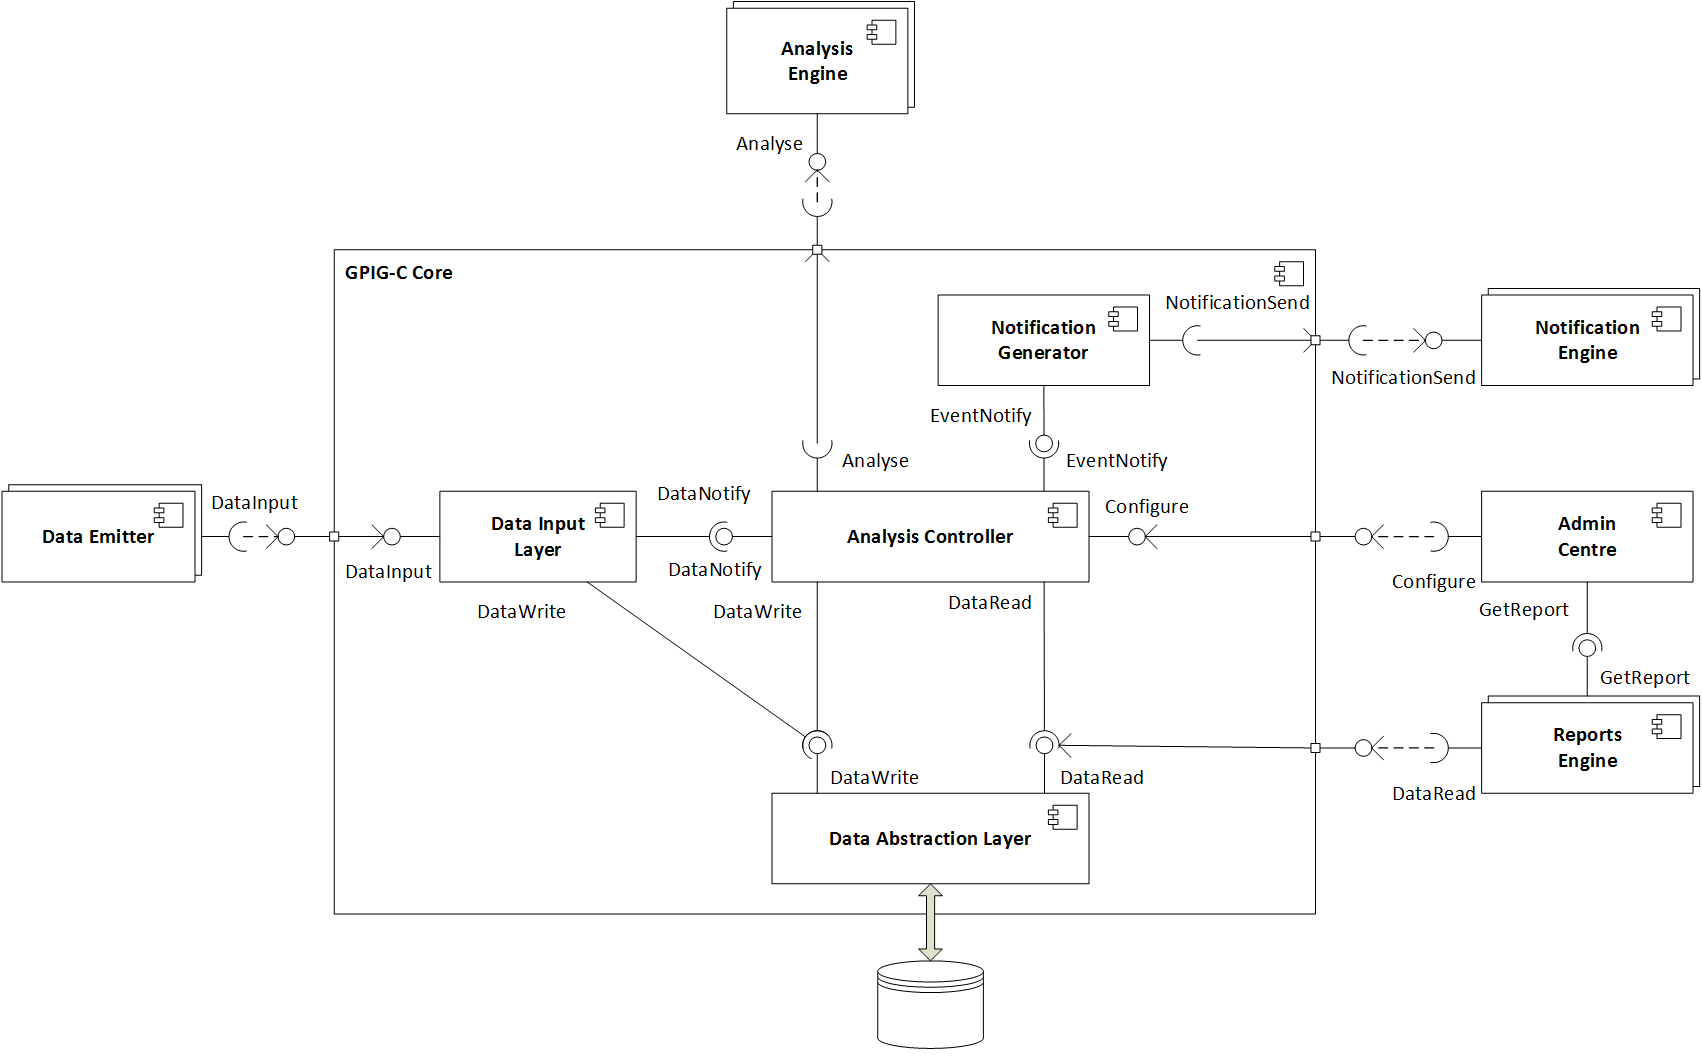
\includegraphics[width=14cm]{images/ComponentDiagram.png}
  \caption{The module diagram of the HUMS}
  \label{fig:ComponentDiagram}
\end{figure}

\begin{description}
  \item[Core] A collection of modules that must be run on one system, including the data input layer, analysis controller, data abstraction layer, and notification generator. Additional modules can be integrated on the same system or connected over a network interface.

  \item[Data Emitter] Sends data to the system core in a standard
    format. May be included within the HUMS or created by the end
    user.

  \item[Data Input Layer] Receives data from a data emitter and sends
    it to the data abstraction layer. Alerts the analysis controller
    that new data was received.

  \item[Data Abstraction Layer] Handles all interaction with the
    database, such that if the database was to be altered, only this
    layer would need to change.

  \item[Analysis Controller] Alert the analysis engines when new data
    has arrived, pulling the required data from the data abstraction
    layer. If an analysis engine determines an event has occurred
    within the data then the analysis controller forwards that event
    to the notification generator.

  \item[Analysis Engine] Analyses the data looking for trends. If a
    trend is found an event is returned to the analysis
    controller. Analysis engines may be included in the HUMS or
    created by the end user.

  \item[Notification Generator] Receives events from the analysis
    controller, defines an abstract notification, and sends it to the
    appropriate notification engine.

  \item[Notification Engine] Receives an abstract notification from
    the notification generator and creates a concrete notification,
    for example an email or triggering a change in system
    behaviour. Notification engines may be included in the HUMS or
    created by the end user.

  \item[Reports Engine] Pulls data from the data abstraction layer and
    formats it into a report, for example a PDF or graph. Report
    engines may be included in the HUMS or created by the end user.
\end{description}

\subsection{Behavioural View}

The module view shows how modules of the system are connected, however 
does not fully represent the interactions between components and the dynamic actions of the system. A behavioural view can be used to detail this information, showing the flow of data and events within the HUMS. Figure \ref{fig:CommunicationDiagram} shows a communication diagram of the 
HUMS, detailing how the HUMS goes from receiving data from a data emitter to generating a notification. The different objects in the system are shown, along with all the interactions and links between them. The messages sent between different parts are shown and labelled with numbers to represent the chronological order in which they occur.

\begin{figure}[!ht]
  \centering
  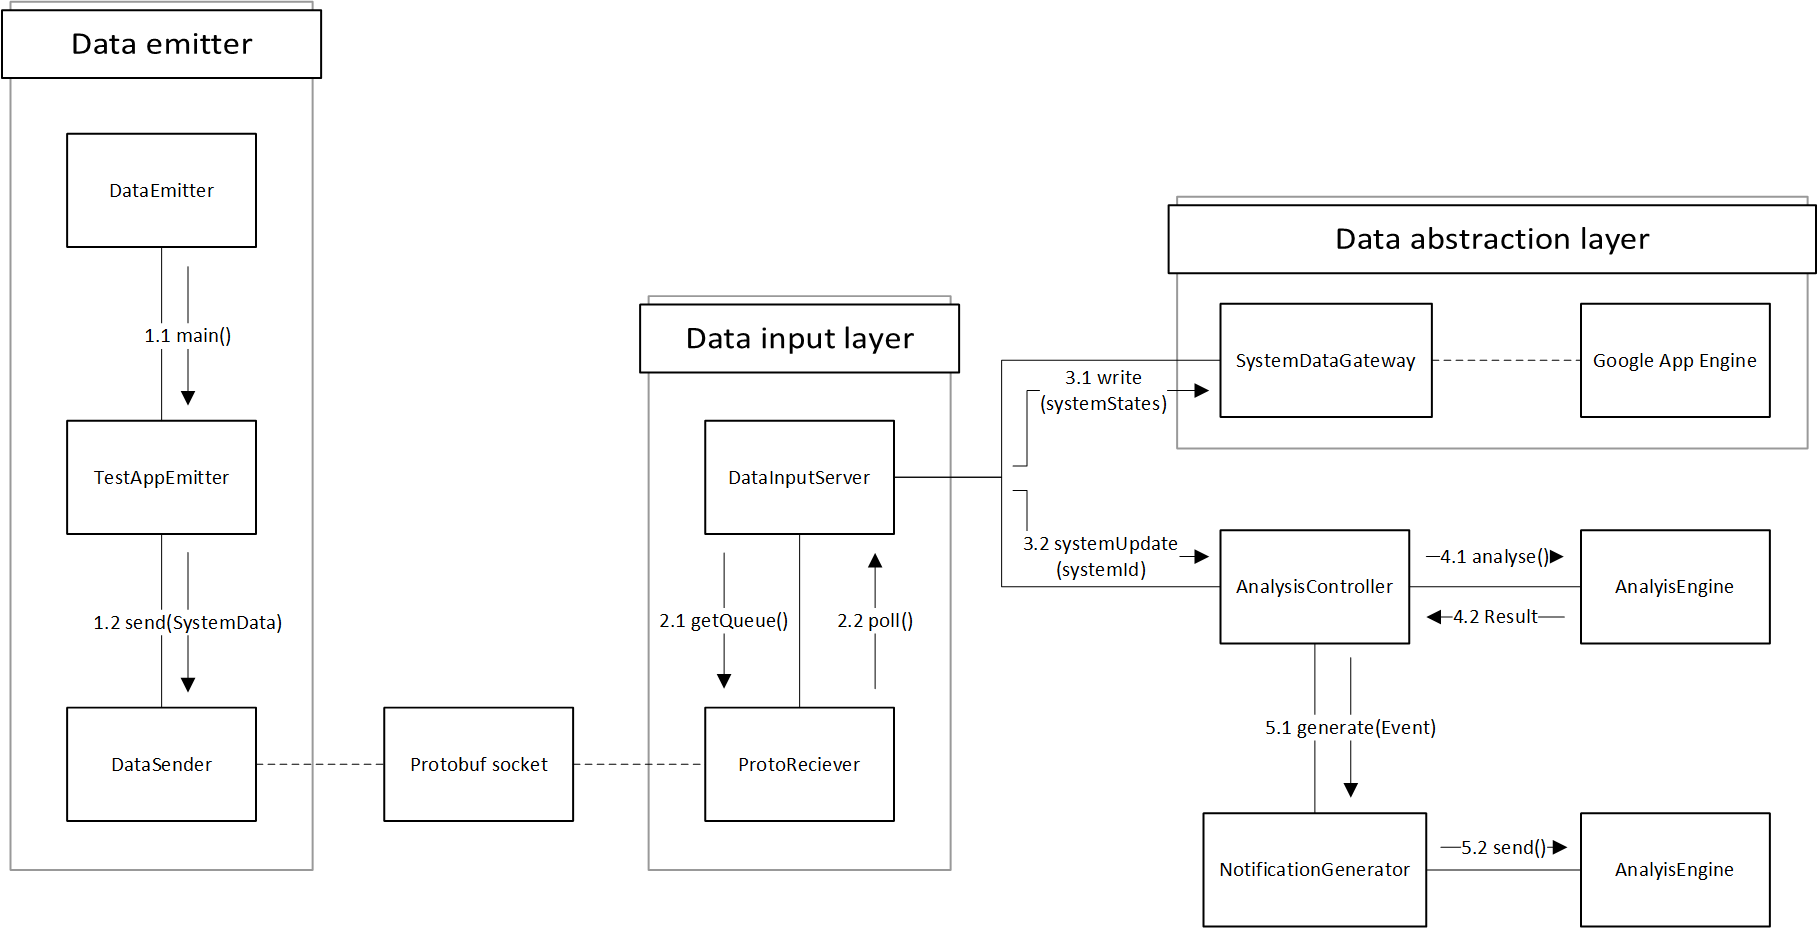
\includegraphics[width=14cm]{images/CommunicationDiagram.png}
  \caption{Communication diagram showing a behavioural view of message 
flow
through the system, using UML 2 notation}
  \label{fig:CommunicationDiagram}
\end{figure}

%%Input Diagram WITH KEY

\subsection{Execution View}
With a view to deployment and execution, the HUMS needs to be tailorable. The core system may be running on the same hardware as the data emitter or it may be geographically distant; engines may be on separate machines or may all be together. Figures \ref{fig:DeploymentDistributed} and \ref{fig:DeploymentIsolated} show the main scenarios for deployment of the HUMS, with a view that if the system architecture can perform under these situations, then it can perform under all others.

Figure \ref{fig:DeploymentDistributed} shows abstractly how the consumer system could be geographically distant to the HUMS core, engines and datastore. It also shows how a remote admin centre could be used, allowing configuration files to be created at a high level by business personel, as opposed to developers. This deployment possibility gave the team the idea of creating a system as a service (SaaS), where multiple customers can simultaneously use a single storage, analysis, and notification server. We felt this was an innovate addition to the HUMS concept as it removes some of the complexity for consumers in setting up and managing their systems, and allows the benefits of cloud computing to be utilised.

This deployment of our HUMS as a SaaS is shown in figure \ref{fig:DeploymentService}. For administering the HUMS as a service, a hosted admin centre will be created, allowing users to specify analysis and reporting behaviours using a simple rules engine-like interface. Users can define their own events and how they should be handled, view all of the registered input clients, pull reports, and view live graphs of data.

Figure \ref{fig:DeploymentIsolated} shows how we envision the prototype HUMS being deployed, with all modules on the same machine. It also shows how the system will be deployed on an embedded system, with configuration files being created manually, without an admin centre, and all modules existing on the same device.
\begin{figure}[!ht]
  \centering
  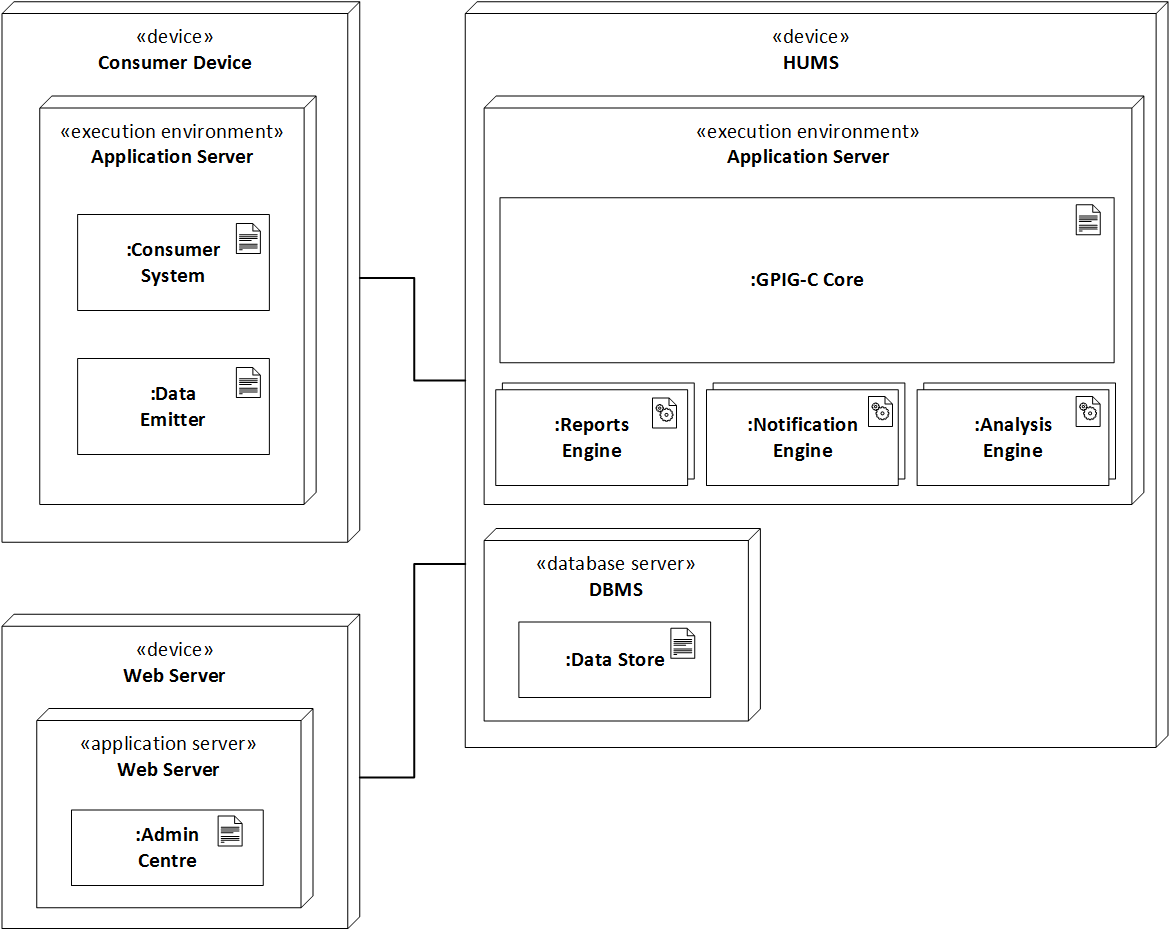
\includegraphics[width=10cm]{images/DeploymentDistributed.png}
  \caption{Deployment diagram showing HUMS spread across multiple 
systems}
  \label{fig:DeploymentDistributed}
\end{figure}

\begin{figure}[!ht]
  \centering
  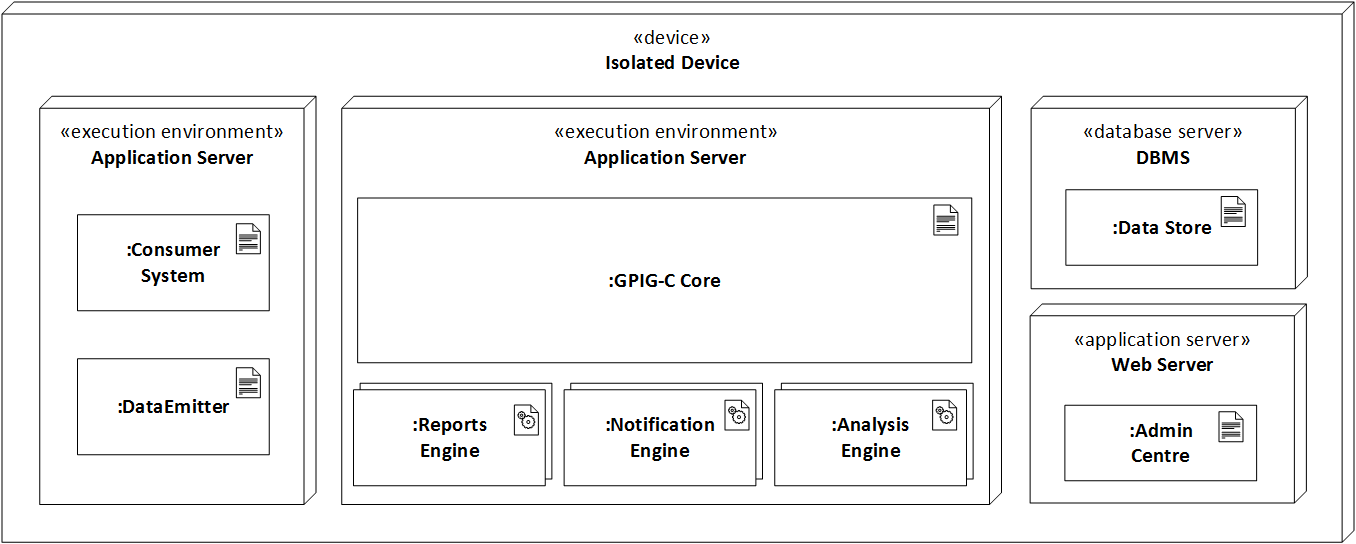
\includegraphics[width=12.5cm]{images/DeploymentIsolated.png}
  \caption{Deployment diagram showing HUMS on one system}
  \label{fig:DeploymentIsolated}
\end{figure}

%
% THIS FIGURE IS NOT REFERENCED ANYWHERE!!
%
\begin{figure}[!ht]
  \centering
  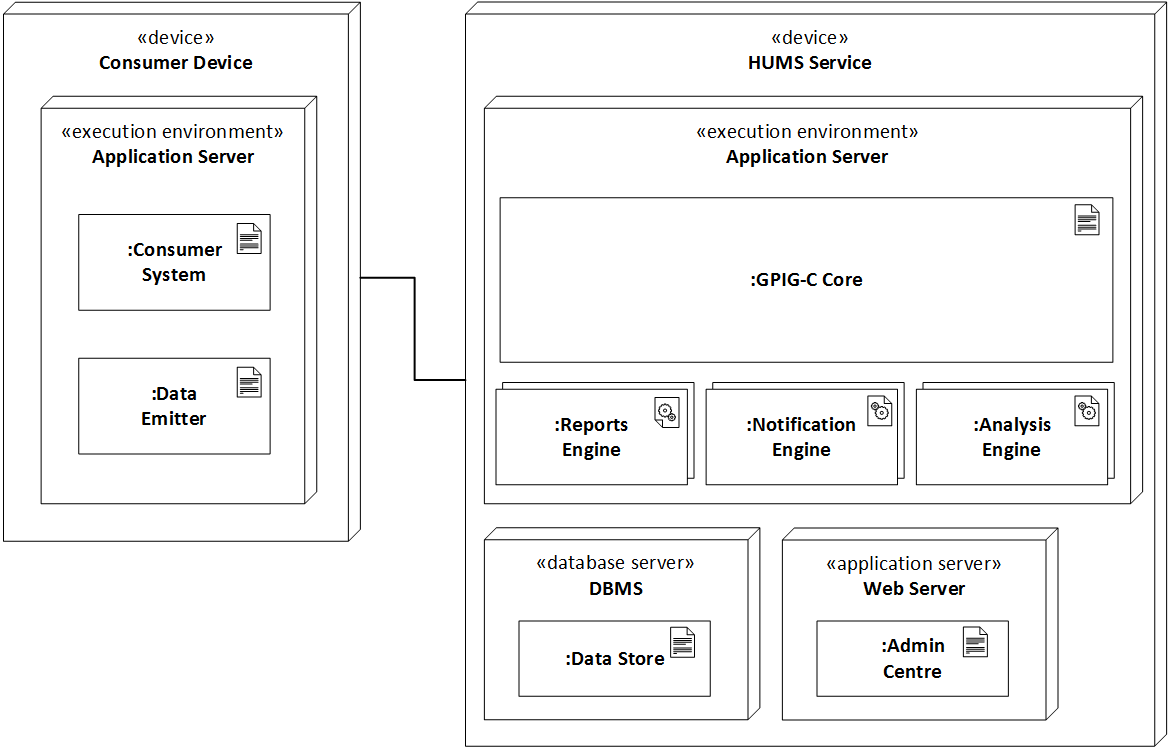
\includegraphics[width=10cm]{images/DeploymentService.png}
  \caption{Deployment diagram showing HUMS as a multi-user service}
  \label{fig:DeploymentService}
\end{figure}

\subsection{Conceptual View}
The conceptual view is a description of the the entire system in terms of its individual components, for example classes in an object-oriented design.

\subsubsection{Data Input Layer}

The data input layer, shown in figure \ref{fig:dataInputLayer},
contains the following classes:

\begin{description}
  \item[DataInputServer] An object which starts up a multithreaded
    server to receive connections, and which periodically processes
    received data by sending it off to the database and notifying the
    analysis component. It accesses these by having references to them
    passed in upon creation.

  \item[ProtoReceiver] Listens on a socket for inbound connections,
    and then hands them off to a new ProtoMultiReceiver, running in a
    new thread, for processing. It also maintains a thread-safe
    concurrent queue, which all of the receivers write to, and the
    server reads (and removes) from. This use of multithreading
    enables multiple clients to send data at the same time easily, and
    the use of a queue ensures that data is inserted into the database
    in the order in which it is received.

  \item[ProtoMultiReceiver] Receives data from a particular data input
    client, writing received data to the queue.
\end{description}

\begin{figure}[ht!]
  \centering
  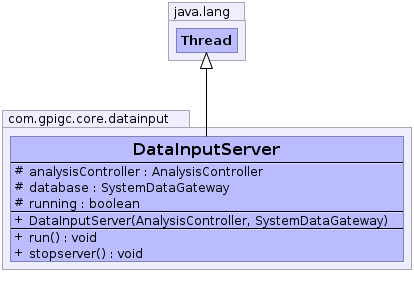
\includegraphics[width=6.2cm]{images/DataInputLayer/DataInputServer.png}
  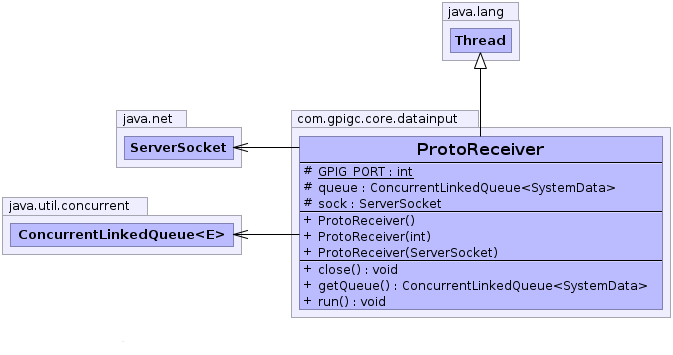
\includegraphics[width=8.3cm]{images/DataInputLayer/ProtoReceiver.png}
  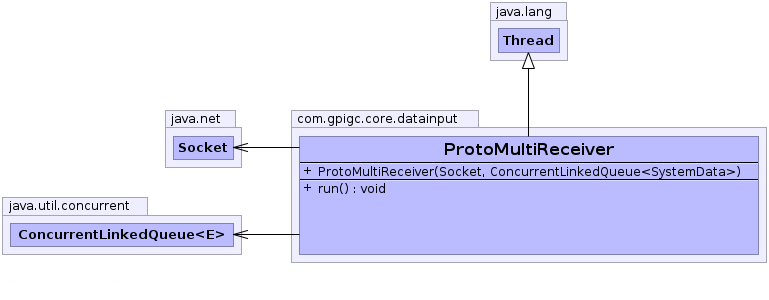
\includegraphics[width=9.5cm]{images/DataInputLayer/ProtoMultiReceiver.png}
  \caption{Conceptual diagrams of the data input layer classes, using 
UML 2 notation}
  \label{fig:dataInputLayer}
\end{figure}

\subsubsection{Data Abstraction Layer}

The data abstraction layer, shown in figure
\ref{fig:dataAbstractionPackage}, contains the following classes:

\begin{description}
  \item [SystemDataGateway] An interface used to abstract the
    datastore implementation details from the rest of the
    application. An implementation of this interface will provide ways
    to read and write from the chosen datastore, meaning the rest of the
    system is not concerned with the datastore implementation. When
    interfacing with a datastore the end user will be required to
    implement this interface.

  \item [EmitterSystemState] An object representing the data received
    from a data emitter at a particular time. The state object holds
    the ID of the end user's system and the creation timestamp along
    with a map of sensor IDs against the value of the sensor at that
    particular time. A map was used to represent the sensors and
    values so that the end user is free to send data from as many or
    as few sensors at a time, reducing the number of writes to the
    database. For serialisation this object includes methods to
    convert to and from JSON.

  \item [DataJSONAttribute] An enumeration that wraps up the keys used
    to look up values in the JSON serialisations of the
    EmitterSystemState and QueryResult classes.

  \item [SensorState] An object representing the state of a particular
    system sensor. A sensor has an ID, a value and two timestamps, one
    specifying the time the sensor value was added to the database and
    the other the time the actual value was sensed or created.

  \item [QueryResult] An object representing the result of a database
    query, containing the ID of the end user's system to which the
    data relates and a list of sensor states pulled from the database.
\end{description}

\begin{figure}[ht!]
  \centering
  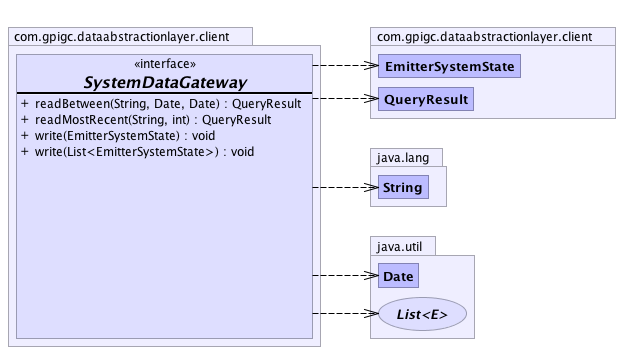
\includegraphics[width= 9.5cm]{images/DataAbstractionLayer/systemDataGateway.png}
  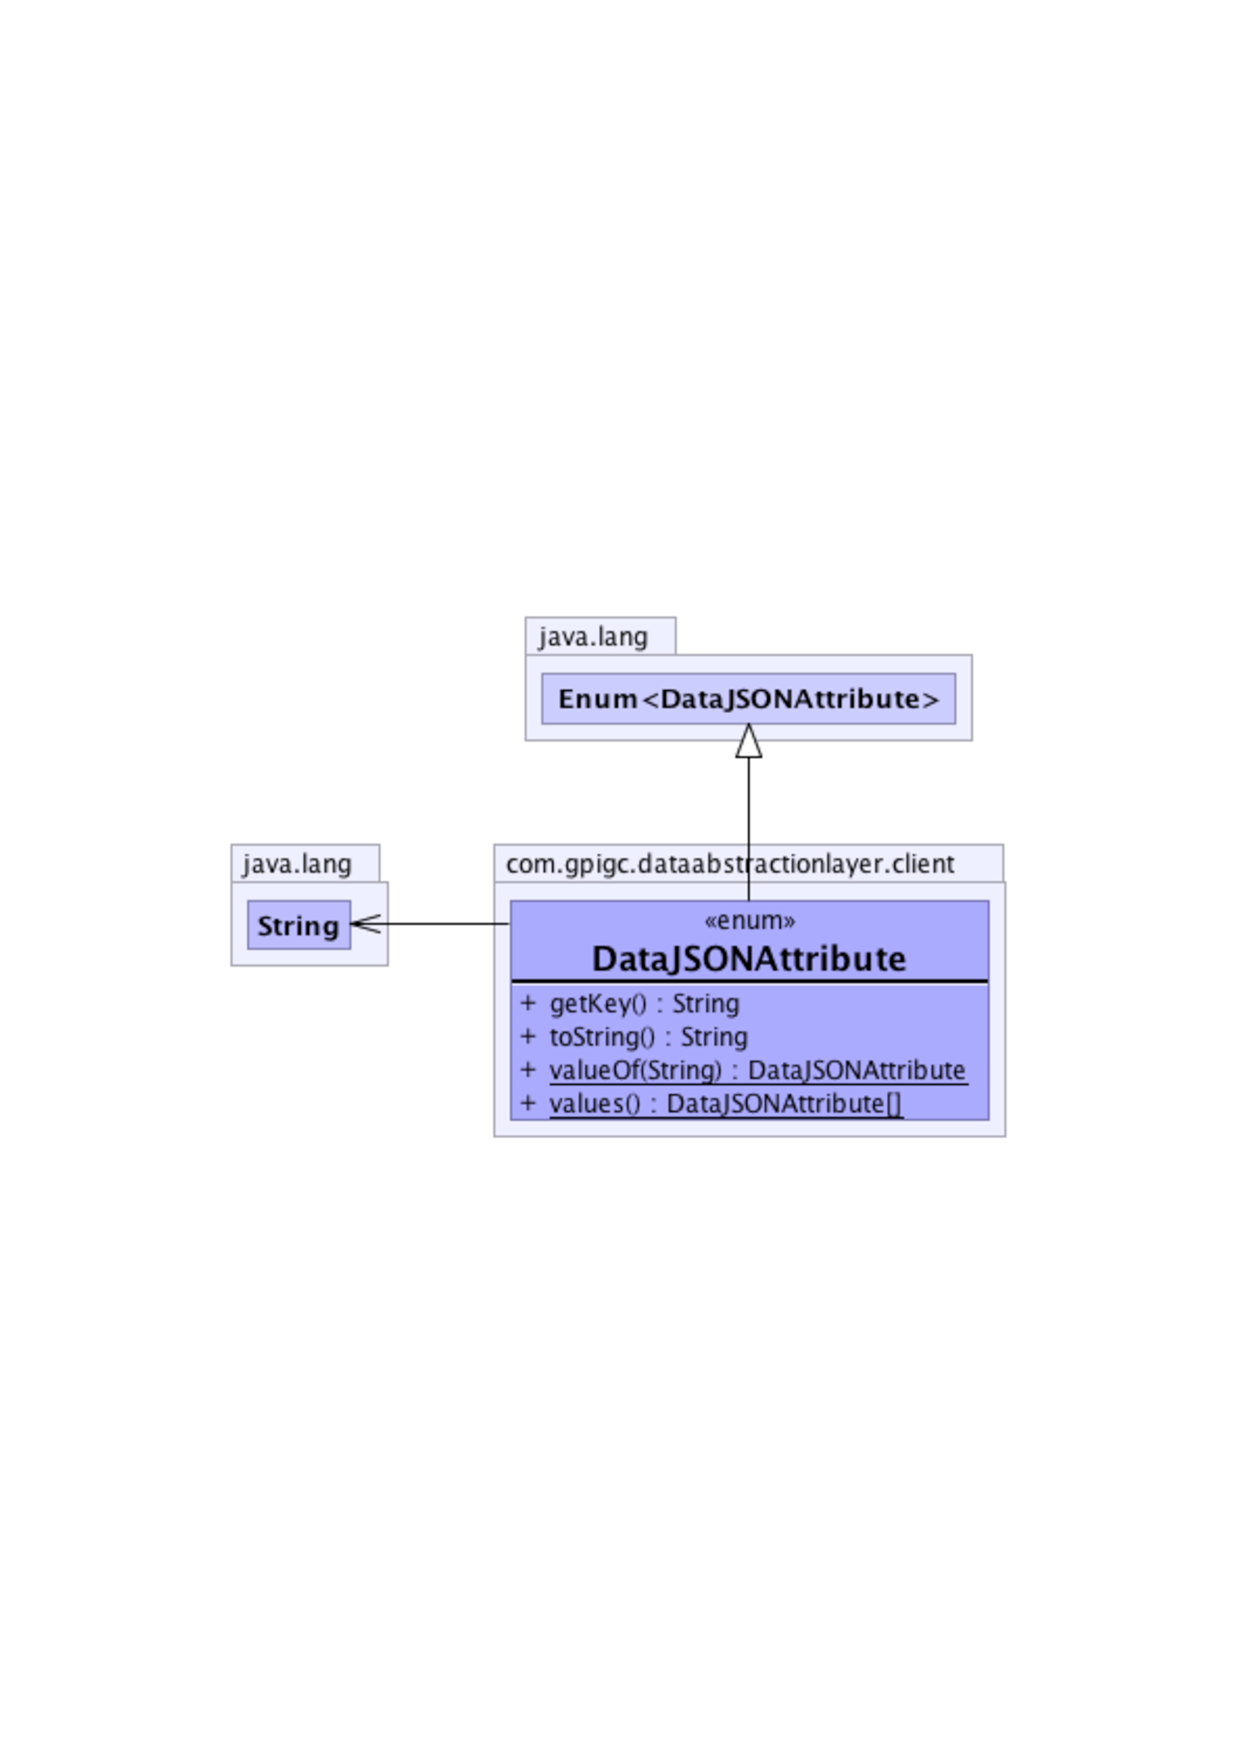
\includegraphics[width= 5cm]{images/DataAbstractionLayer/dataJsonAttribute.pdf}
  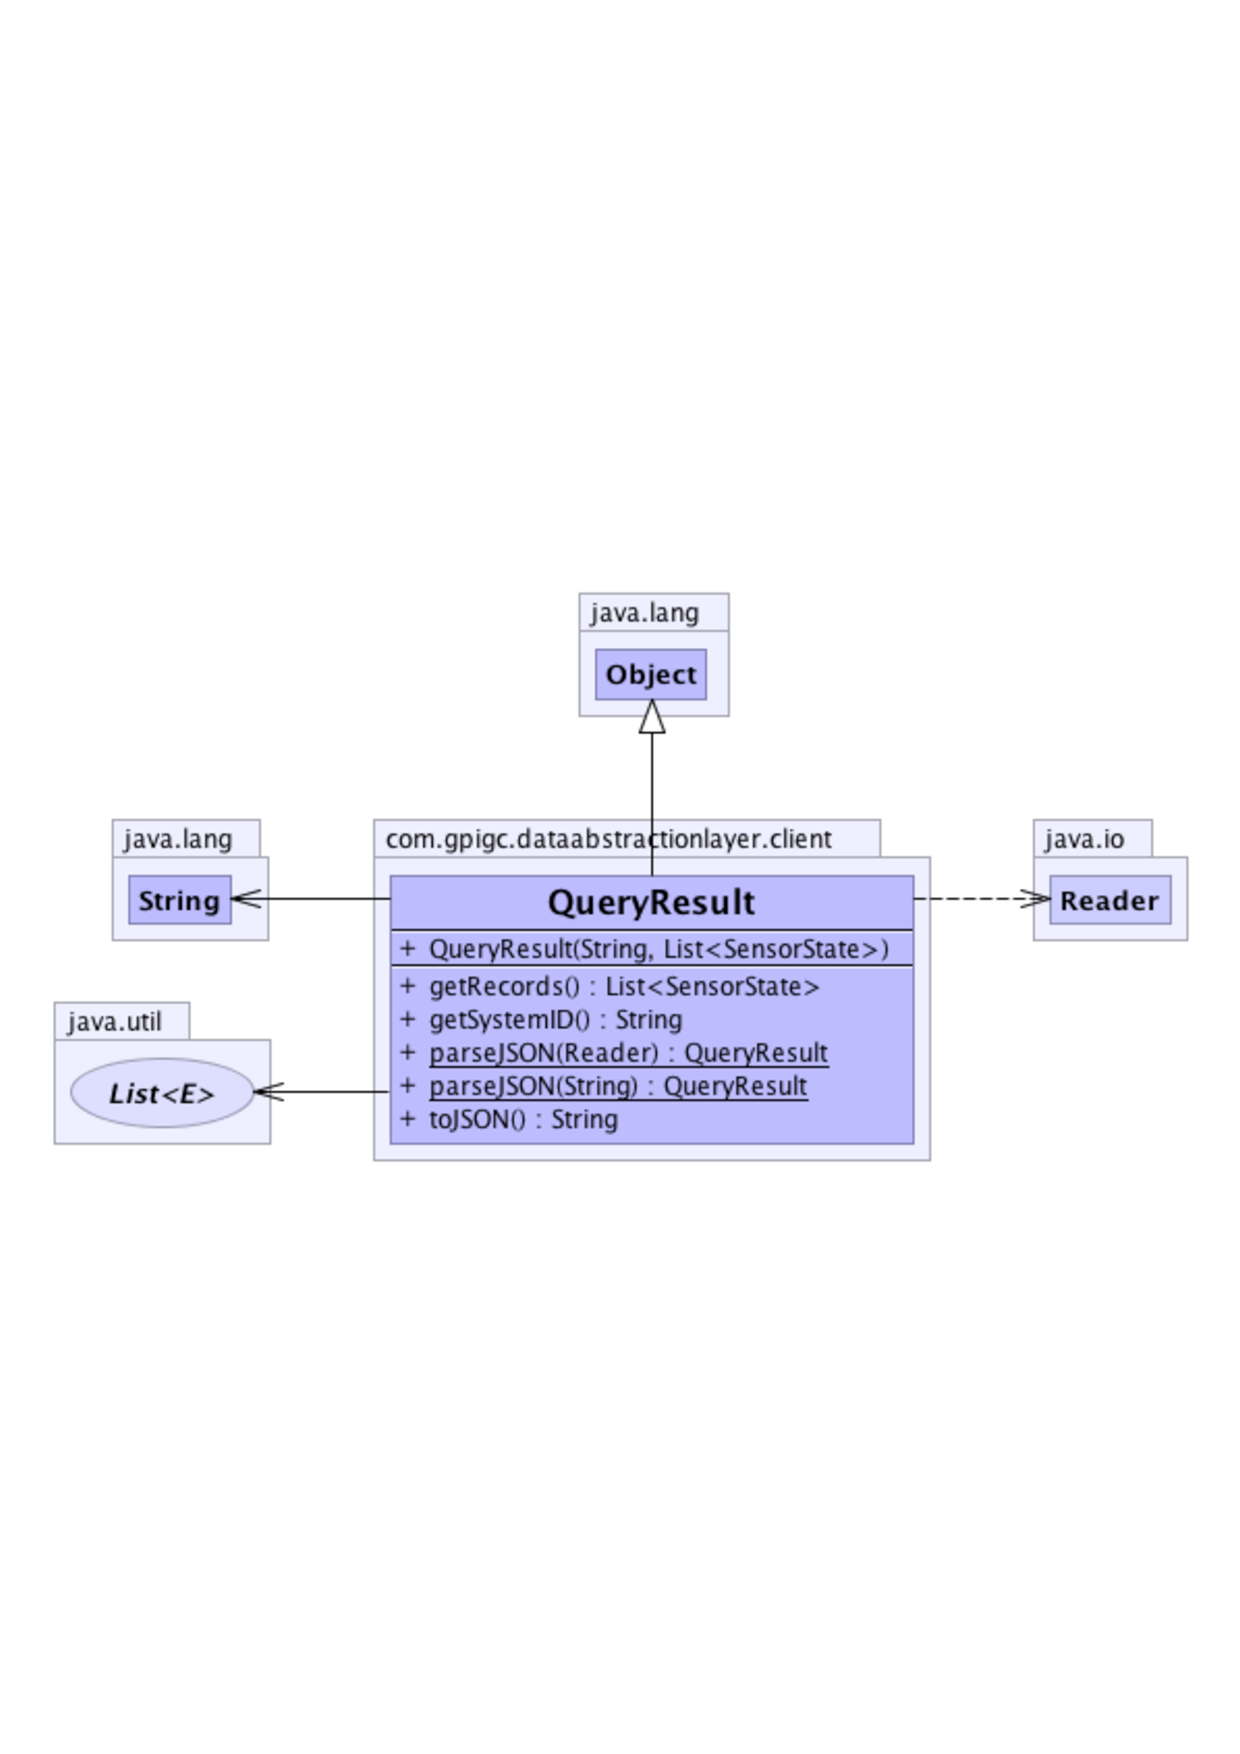
\includegraphics[width= 7cm]{images/DataAbstractionLayer/queryResult.pdf}
  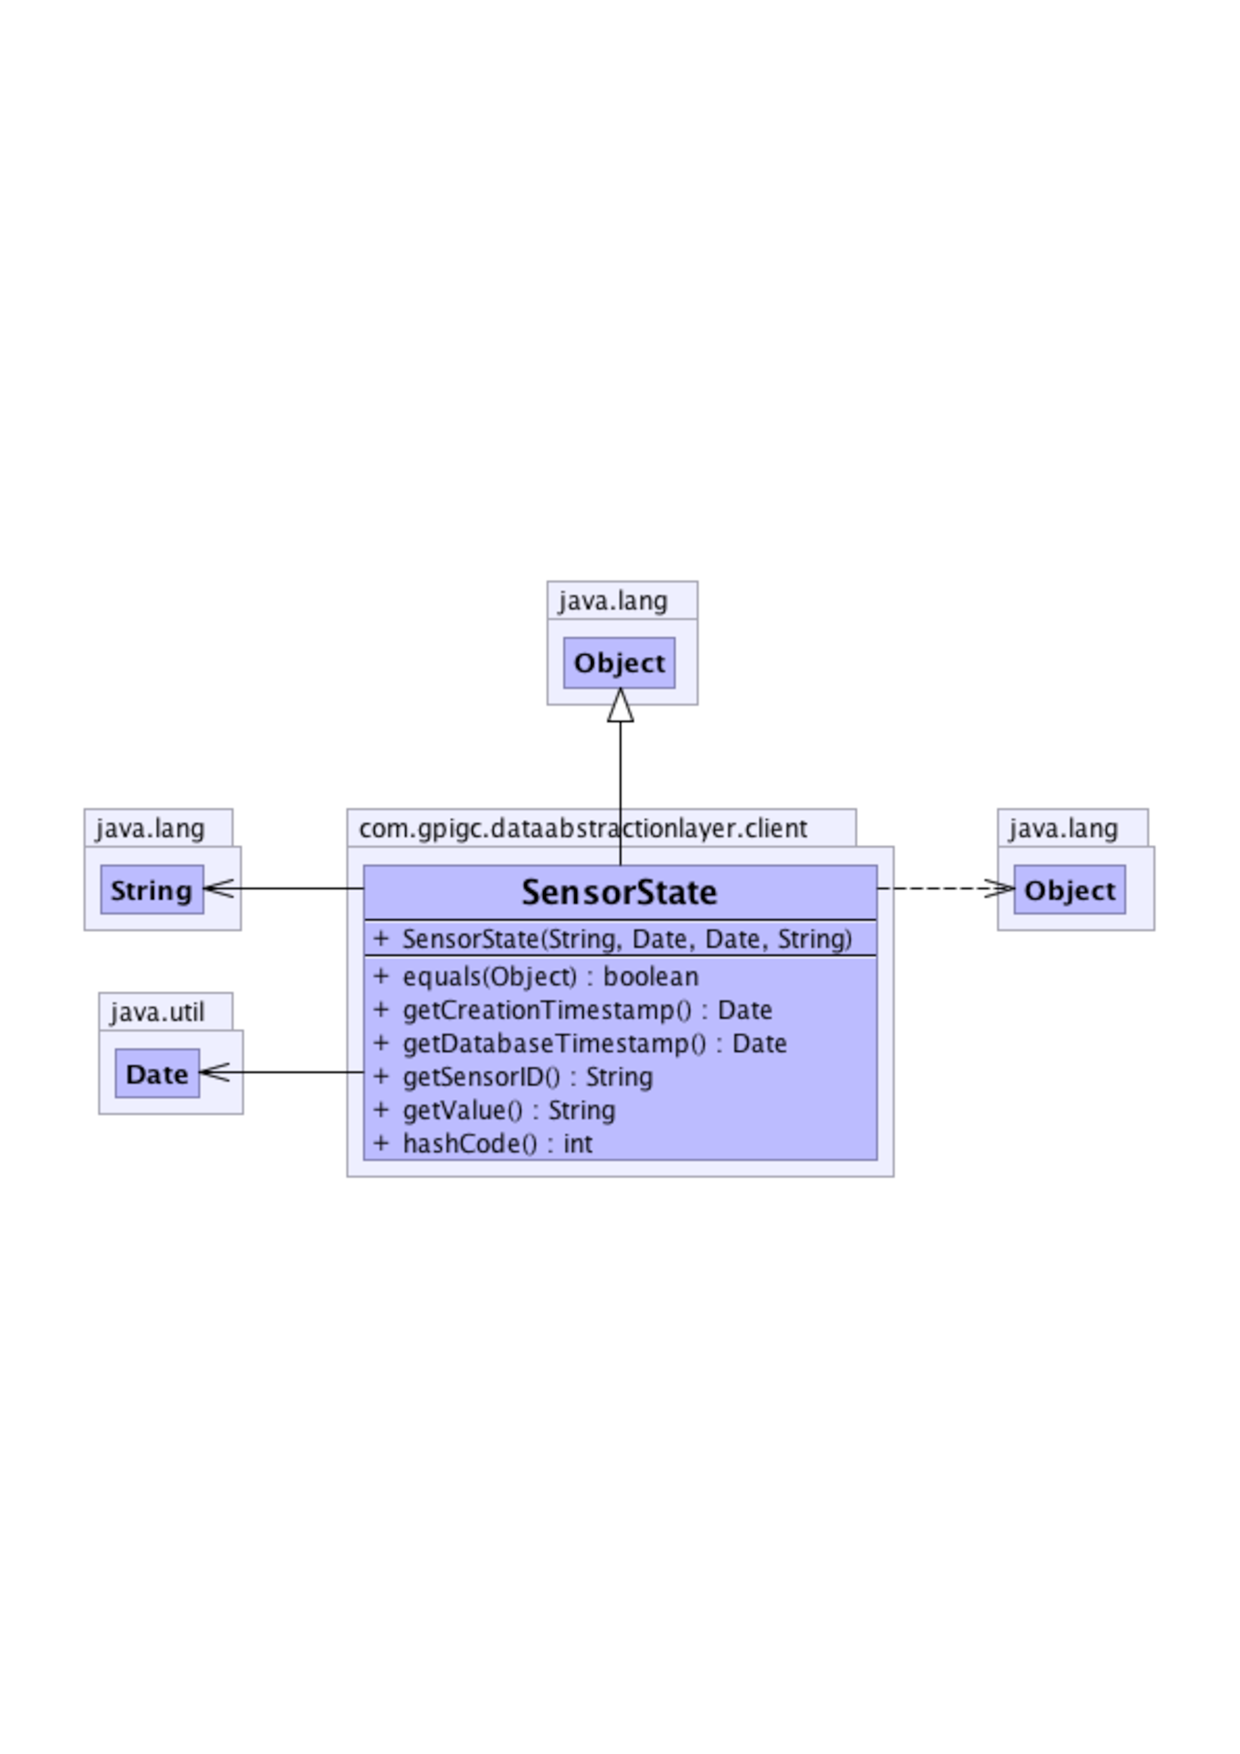
\includegraphics[width= 7cm]{images/DataAbstractionLayer/sensorState.pdf}
  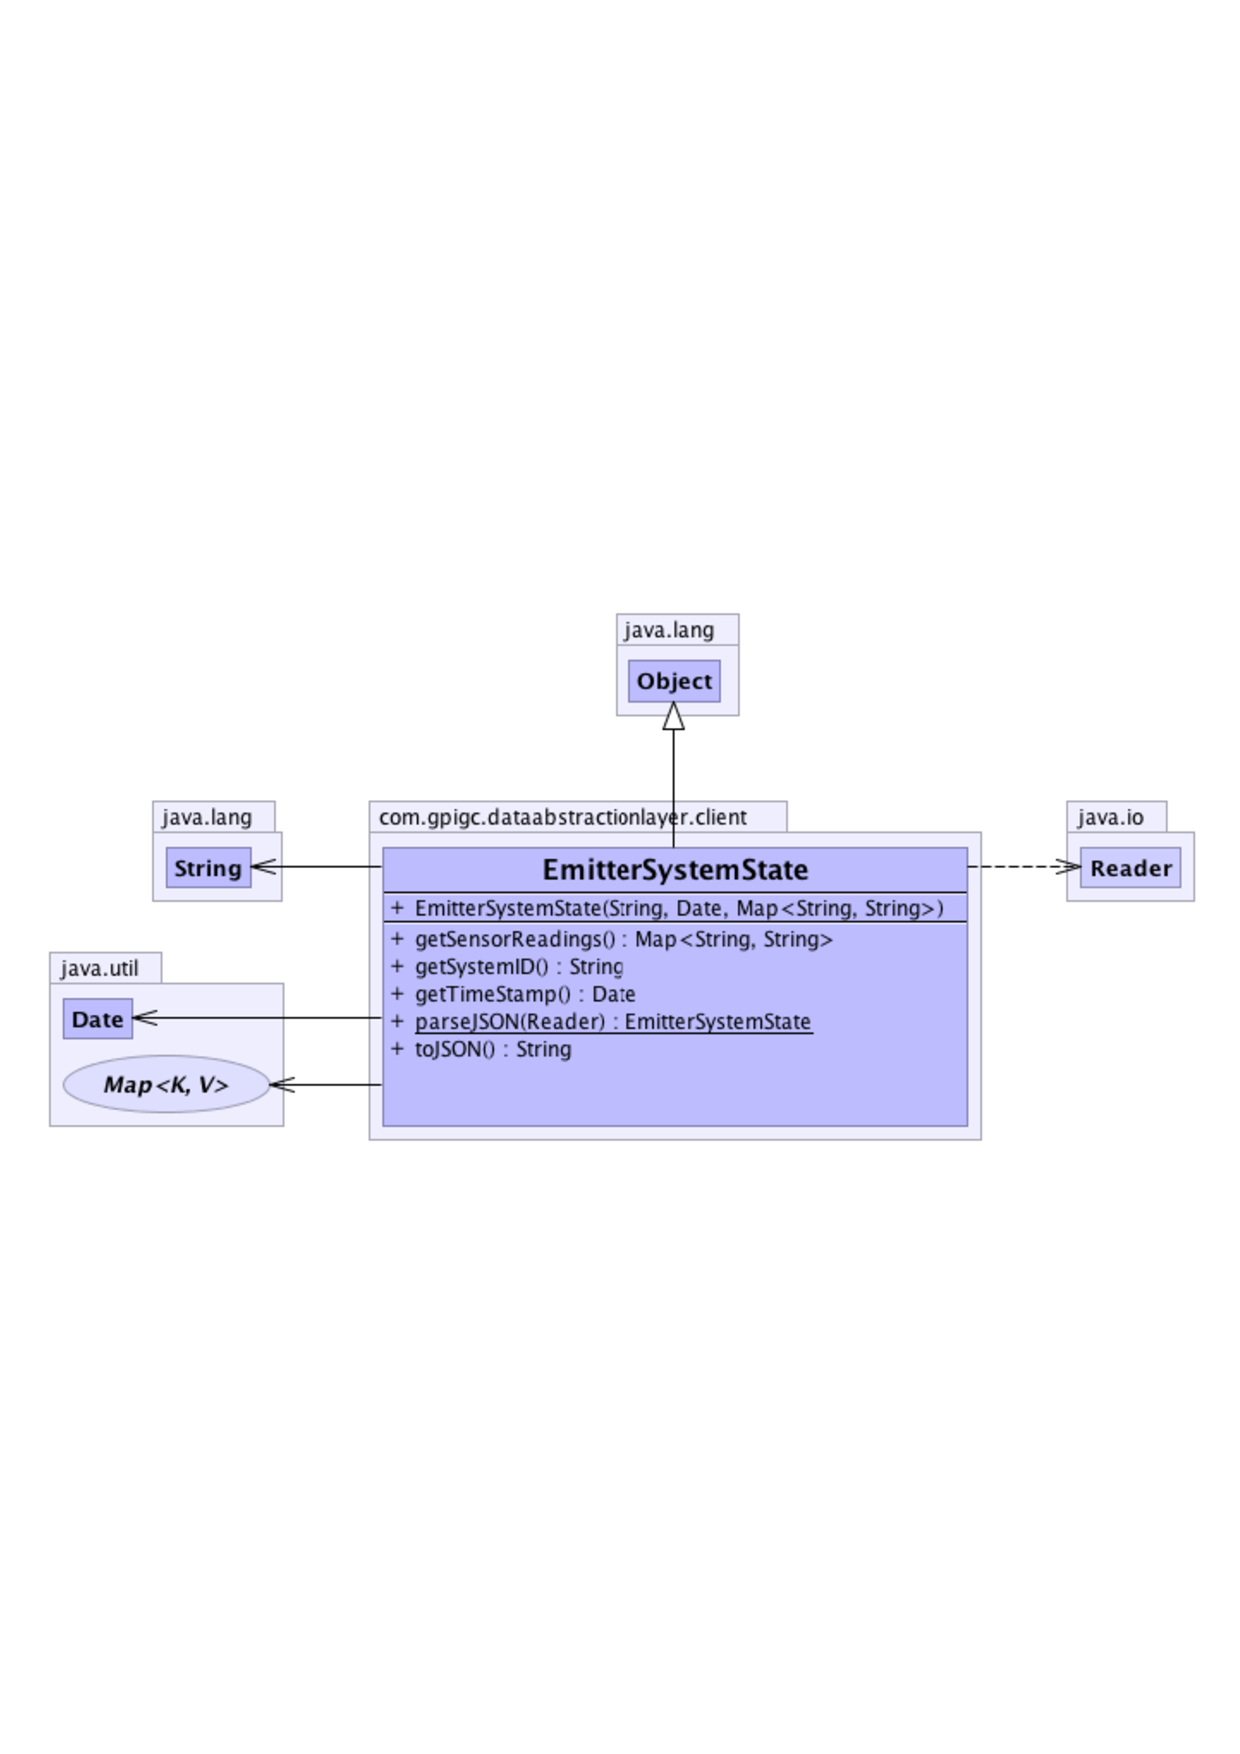
\includegraphics[width= 9cm]{images/DataAbstractionLayer/emitterSystemState.pdf}
  \caption{Conceptual diagrams of the data abstraction layer classes, 
using UML 2 notation}
  \label{fig:dataAbstractionPackage}
\end{figure}

\subsubsection{Analysis Components}

The analysis component, shown in figure
\ref{fig:dataAnalysisComponent}, contains the following classes:

\begin{description}
  \item [AnalysisController] An object that coordinates all analysis of
    sensor data. The object interfaces with the data input layer,
    receiving a system ID when analysis is required. Once analysis has
    been carried out the controller processes the results and triggers
    notifications where appropriate. Analysis engines are associated
    with the analysis controller by class loading allowing for users to
    add and remove analysis engines at run-time.

  \item [AnalysisEngine] An abstract class that implements the basic
    functionality and defines the methods required of an implemented
    analysis engine. Each engine has a list of associated systems. The
    implementation of the analyse method interfaces with the database
    abstraction layer to retrieve the appropriate sensor data and then
    performs the desired analysis. Once analysis is complete the engine 
    returns a result object. When creating their own analysis 
    engines the end user will be required to extend this class, implement 
    the abstract methods and define what constitutes an event.

  \item [MeanAnalysis] An object that extends the analysis engine
    class and implements mean analysis. When called by the analysis
    controller, sensor data is retrieved for all associated systems
    and mean analysis is performed. If a mean value falls outside of
    the acceptable bounds then a flag is set to generate a notification.

  \item [Result] An object representing the result of the analysis
    carried out by the chosen analysis engine. The object contains a
    map of any data to be saved back to the database and a flag
    indicating whether a notification needs to be triggered. For
    serialisation the data to be saved to the database is stored in a
    map of string key-values. When implementing their own analysis
    engine the end user will be able to specify what data is to be
    saved back to the database.

  \item [Event] An object representing an event,
    containing the name of the analysis engine that triggered the
    event, the ID of the system that the event applies
    to, and the result object from the analysis engine that triggered
    the event.
\end{description}

\begin{figure}[ht!]
  \centering
  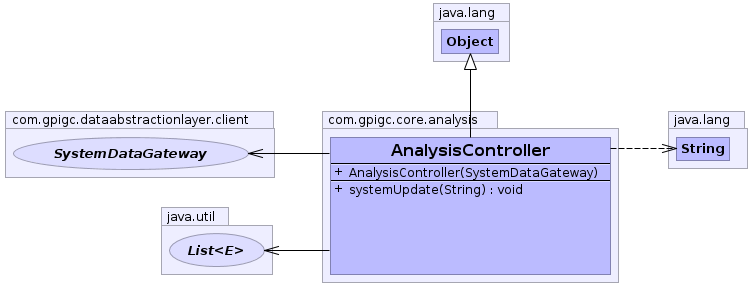
\includegraphics[width= 9.5cm]{images/Analysis/AnalysisController.png}
  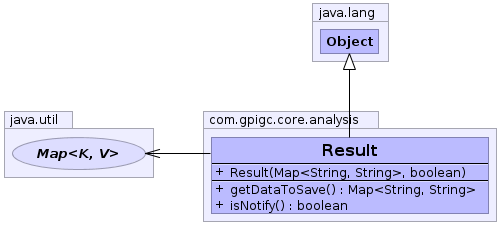
\includegraphics[width= 5cm]{images/Analysis/Result.png}
  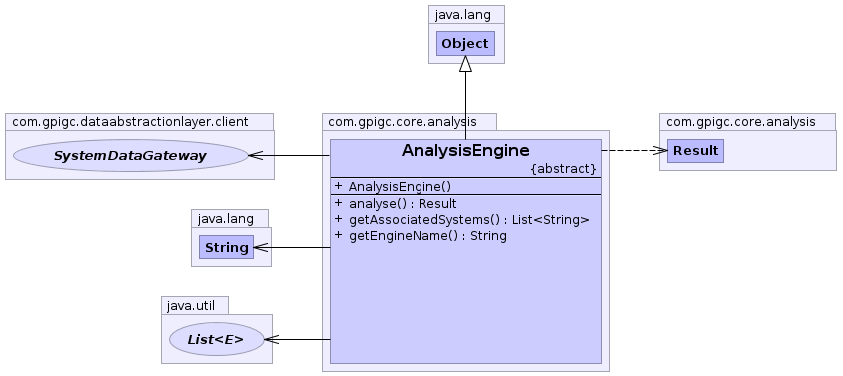
\includegraphics[width= 12cm]{images/Analysis/AnalysisEngine.png}
  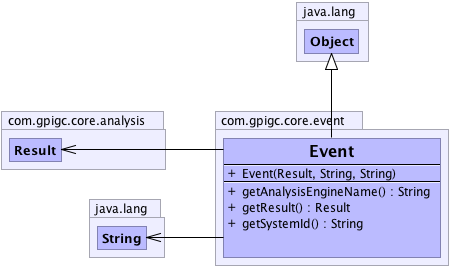
\includegraphics[width= 6cm]{images/Analysis/Event.png}
  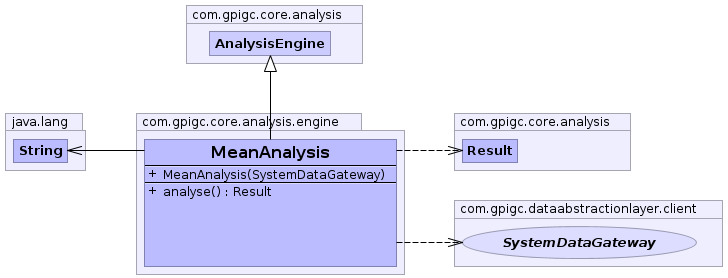
\includegraphics[width= 8cm]{images/Analysis/MeanAnalysis.png}
  \caption{Conceptual diagrams of the analysis component classes, using 
UML 2 notation}
  \label{fig:dataAnalysisComponent}
\end{figure}

\subsubsection{Notification Components}

The notification component, shown in figure
\ref{fig:notificationComponent}, contains the following classes:

\begin{description}
  \item [NotificationGenerator] An object that coordinates generating and
    sending of notifications. The object interfaces with the analysis
    controller, receiving an event object when analysis engines specify that
    notifications should be sent. Notifications are then generated and sent by
    appropriate notification engines. Notification engines are associated with
    the notification generator by class loading allowing for users to add and
    remove notification engines at run-time.

  \item [NotificationEngine] An abstract class that implements the basic
    functionality and defines the methods required of an implemented
    notification engine. Each engine has a list of associated systems, and 
    features a cool down system to ensure that notifications are not sent
    more then once during a specified period of time. When creating their
    own notification engines the end user will be required to extend this
    class, implement the abstract methods, and define how a notification
    is sent.

  \item [EmailNotification] An object that extends the notification engine
    class and implements email notifications. When called by the notification
    generator, an email notification is sent to the specified recipient, and 
    contains the specified notification subject and further notification
    information.
\end{description}
 
\begin{figure}[ht!]
  \centering
  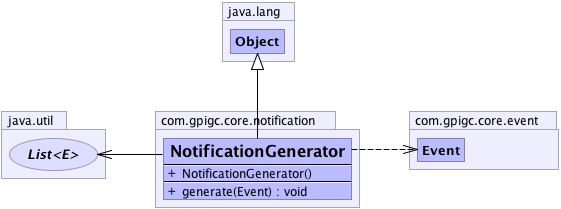
\includegraphics[width= 7cm]{images/Notification/NotificationGenerator.png}
  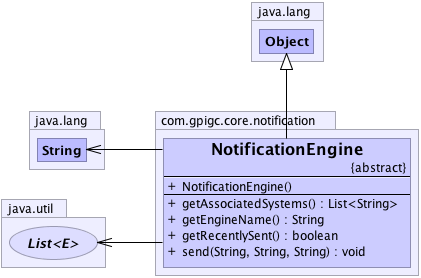
\includegraphics[width= 5cm]{images/Notification/NotificationEngine.png}
  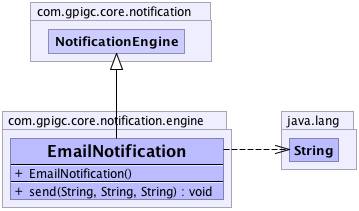
\includegraphics[width= 4.5cm]{images/Notification/EmailNotification.png}
  \caption{Conceptual diagrams of the notification component classes, using 
UML 2 notation}
  \label{fig:notificationComponent}
\end{figure}

\section{Interim Prototype Implementation}

\subsection{Technologies}

We chose to develop the core of the HUMS prototype in Java. Java can
be compiled to bytecode that can be executed directly in all
environments that support a Java Virtual Machine, including various
operating systems and the x86, x86-64 and ARM CPU architectures,
making it highly portable between both desktop, server and embedded
systems. % REF: http://www.oracle.com/technetwork/java/javase/config-417990.html

Whilst there may exist deployment platforms that are not supported, at
this stage, we do not see this as a problem since the underlying
architecture of the system is transferable across languages.

All members of our team were familiar with the Java programming
language and thus no time was spent having to get the team up to speed
on a new language. We did not impose a language restriction when
developing the data emitter and various engines as the data being
passed between them and the core are language independent, meaning 
end users are free, even with the prototype, to implement engines in any
language they see fit. For the prototype we used both Java and
JavaScript when creating the engines---languages that team members are
familiar with---allowing us to show off the versatility of the system.

Upon deciding to monitor CPU and heap usage, we began to investigate
technologies that would allow us to do so, rather than reinvent the wheel.
Doing this also had the benefit of providing us with established, well-tested
tools with which we could easily implement data input clients for further
systems. As the test program is a Java program, we had to connect to its JVM to query the heap usage, as the operating system would just report the size of the JVM heap. We settled on using SIGAR for process monitoring, and JMX for monitoring heap usage.

An alternative we considered was simply querying the existing features provided
by the operating system and JVM to access this data, however this would have
not been portable across different operating systems, or to embedded systems
with poor support for launching new processes.

To communicate between the core and the other modules, we serialised objects to send them over a network connection. We used JSON and Protocol Buffers. For connections that require data to be serialised to text, we used JSON since it is human readable and maps well to our internal representation of objects in Java. To read and write JSON we used the Jackson library, since it offers a high-performance streaming API. When there was no such restriction on the format of the transmitted data, we used Google Protocol Buffers since they offer high performance, as is necessary for the potentially high-volume connections between the Core and the other modules, such as the Data Emitter and the Analysis Engines.

We initially considered using HTTP rather than Google Protocol Buffers for
communication between the data input layer and the core, however we determined
that sending multiple HTTP requests a second would have significant overhead,
and so we instead opted for a persistent connection and a more lightweight
protocol.

We chose to use Google App Engine to host the prototype's database
module, displaying how easily it can incorporate existing, popular
technologies as plugins. The prototype could easily be extended to
work with other database technologies simply by implementing an
interface within the data abstraction layer.

We created a prototype admin centre to show how the HUMS could be
managed remotely, viewing data and modifying settings online, through
a web browser, whilst running as a service. The admin centre was
developed using the Bootstrap front-end web framework, including 
HTML, JavaScript and CSS, in order to create a prototype realistically
simulating an interface to the HUMS that is accessible on desktop
computers, laptops and mobile devices alike.

We used various Java libraries to support our prototype, saving us 
development time and providing a robust codebase. For testing we used 
the Mockito framework to allow us to verify elements of our codebase in 
isolation, by offering a concise way to mock out dependancies.

We used Git for version control, allowing the entire team to
contribute to the project simultaneously, whilst keeping a reversible
history of all alterations made by each person. We considered using a
centralised version control system, such as Subversion, but decided that the
benefits provided by a decentralised system, such as Git, for working
independently and then combining work would outweigh the potential
disadvantages of there being no managing server. As we used GitHub for the
canonical copy of the work, we incorporated many of the benefits of centralised
version control anyway.

\subsection{Current Functionality}
For the interim prototype we chose to firmly follow the planned architecture, producing a core system linking to example engines, emitters and data stores, focussing on interacting with the provided test application.

The core of the HUMS is fully functional, allowing for data emitters to send data to the data input layer using protocol buffers, chosen in preference to HTTP requests due to the lower latency. The data input layer, as currently implemented, supports multiple simultaneous connections from input clients, although we have yet to investigate how many the prototype could handle. Upon receipt, the data is put into a queue, which is periodically processed by the data input server, by adding each entry to the database and notifying the analysis controller. The analysis controller allows for dynamic loading of analysis engines, allowing them to be altered at runtime and requests data to be passed to the appropriate engine, decoupling the analysis engines from the data abstraction layer. The data abstraction layer provides a simple interface to be implemented by the consumer and includes an example implementation, interfacing with Google App Engine using HTTP requests to a remote servlet. The notification generator also allows notification engines to be dynamically loaded and passes event objects to them.

Currently there are two data emitters for use with the system. Demoing its flexibility, the first extracts and emits data about the JVM, recording CPU and memory usage, and the second extracts and emits live data about earthquake activity from the USGS earthquake hazards program API \cite{usgs}.

The data emitter designed to emit data about the JVM records the CPU and memory usage and sends these through the data input API every second. A period of four seconds is allowed to elapse before the first send, allowing the CPU usage readings to stabilise. The data emitter created to relay live data about earthquake activity fetches data every minute from the USGS earthquake hazards program API and submits it to the data input API.

%%Paragraph about analysis plugin 

When the notification generator receives an event, it selects the appropriate notification engines for that event and uses them to create and send a notification. Currently, a single notification engine has been developed which sends an email to an email address configured by the user. This is demonstrated for the test application, where an email will be dispatched when CPU usage exceeds a predefined limit.

%% Paragraph about reports plugins

A prototype admin centre was created for this stage of the project to demonstrate how the HUMS could be public facing as a SaaS, allowing for any company or individual to, for a fee, use the facilities provided; including storage, analysis, notification and reporting tools. Currently the prototype admin centre mocks functionality and --- apart from the reporting examples --- does not actually integrate with the system. We envisage that in the next phase of the project the admin centre will be functional.

\subsection{Source}
The source for our prototype implementation can be accessed online at \textit{http://git.gpigc.co.uk} and cloned using Git from \textit{http://git.gpigc.co.uk/gpig-c.git}. The username required is \textit{gpigc} with the password \textit{moustache}.

\subsection{Evaluation of the Prototype Solution for Sample Applications}
\label{sec:prototype-evaluation}

\subsubsection{Customer Test Application -- No. 1}
The Customer provided an example application to monitor as part of the
evaluation of our prototype. With this in mind, we created a monitoring 
package for our prototype solution that can monitor a native application
or one executing on the JVM. We utilised Java Management 
Extensions (JMX) to sample the memory utilisation of the application and
created a process monitoring class which monitors the total
CPU usage of the application. The mean analysis engine computes a 
rolling average of values, and causes an email to be sent if this value
becomes too high, as shown in figure \ref{fig:alerting}. The raw memory
values are read by the reporting system and displayed live in the admin
centre, as shown in figure~\ref{fig:graphing}. The graph shows a value from
every 10 seconds, and automatically updates with the latest values.

% Mean - email
% Raw values - graph

\begin{figure}[htbp!]
  \centering
  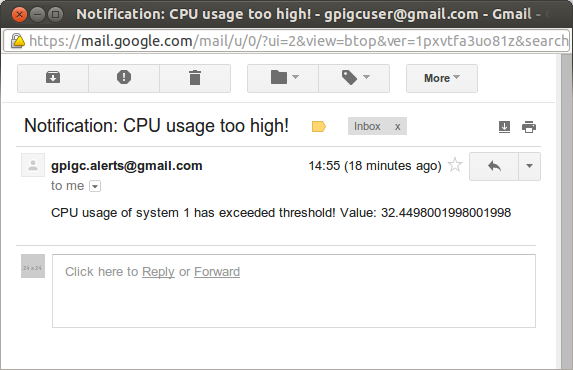
\includegraphics[width=7cm]{images/TestApplicationCPUAlert.png}
  \caption{A screenshot of an email notification sent by the mean analysis engine}
  \label{fig:alerting}
\end{figure}

% TODO Talk about performance or meeting the requirements - we've not implemented quite a few things such as feedback?
\begin{figure}[htbp!]
  \centering
  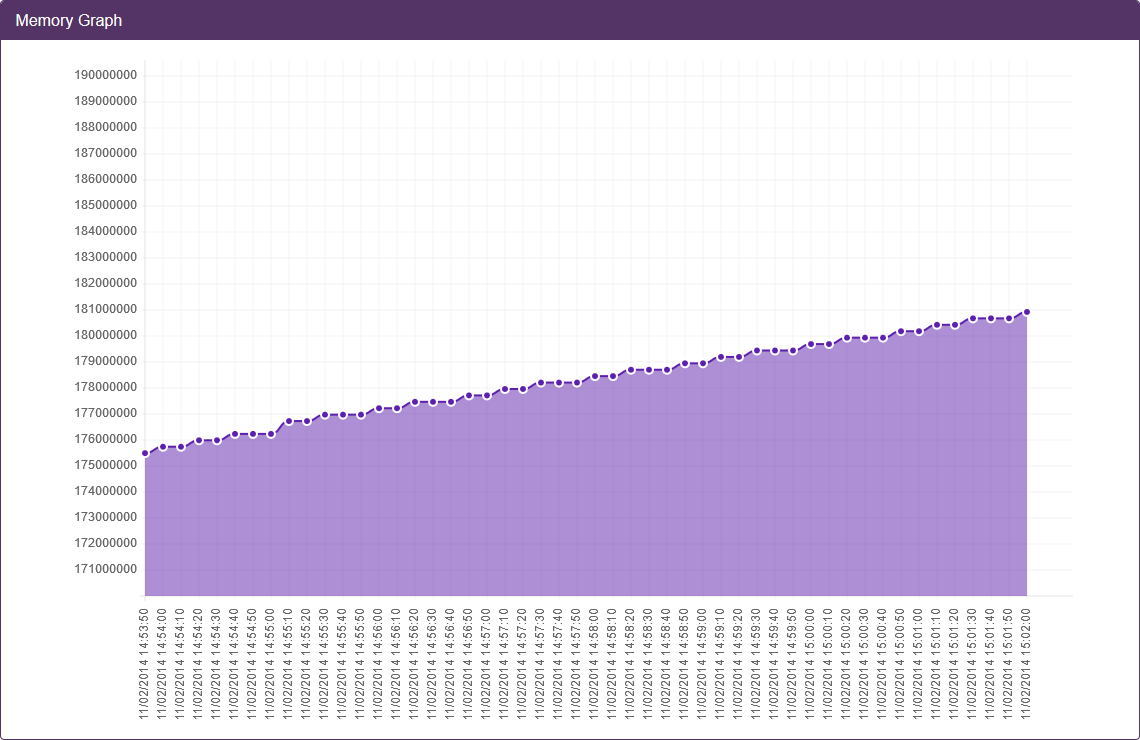
\includegraphics[width=12cm]{images/TestApplicationMemoryGraph.png}
  \caption{A screenshot of the live graphing of the memory usage of the Customer 
  Test Application}
  \label{fig:graphing}
\end{figure}

\subsubsection{Earthquake}
We also created our own sample application: monitoring earthquakes 
through the USGS Earthquake Hazards Program API. The HUMS
can collect live data from the API, store it and plot the location of any
detected earthquakes on a map of the world in the admin centre, as shown
in figure~\ref{fig:plotearthquakes}. We felt that using a map to display
data was a useful and innovative addition.

\begin{figure}[htbp!]
  \centering
  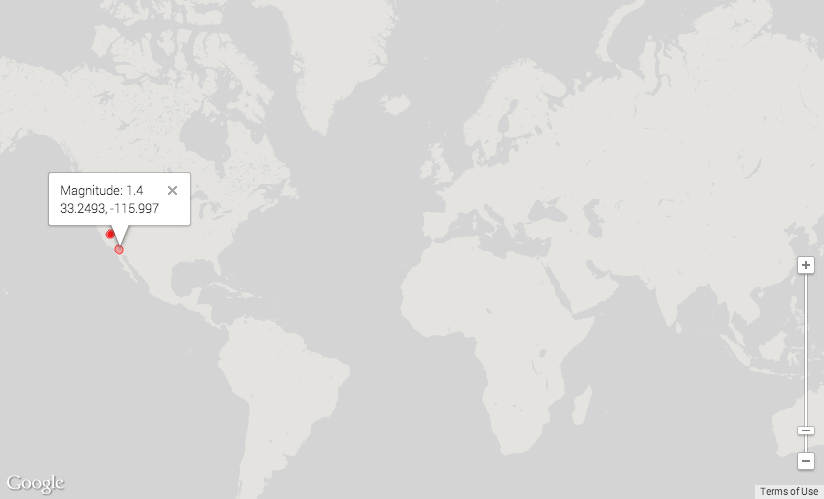
\includegraphics[width=10cm]{images/plotearthquakes.png}
  \caption{A screenshot of the admin centre for our live earthquake monitoring HUMS prototype}
  \label{fig:plotearthquakes}
\end{figure}

\subsubsection{Instructions for Running and Replicating Results}
Once the source has been obtained, it can be run as follows: \hl{Todo - instructions for running the system as a whole: jars and stuff. Joe?}

\begin{enumerate}
  \item Run X with parameters Y, Z in W
  \item Observe result
  \item ????
  \item PROFIT
\end{enumerate}

The test application memory graph can be viewed at \textit{http://www.gpigc.co.uk/admin/graph.html} and the earthquake map can be viewed at \textit{http://www.gpigc.co.uk/admin/map.html}.

\subsection{Testing} 
We created and implemented a test plan that laid out our key ideas
with respect to verifying that our solution fulfilled its
requirements. In this section we give the mapping between each
test and its associated requirement. We
defined our plan, where appropriate, in terms of each module within
the system and what specific, testable attributes that module must
have to fulfil its requirements. We also further deconstructed the
testing into various levels of abstraction, mapping the higher level
requirements to their lower level requisite requirements: acceptance
testing, system testing, integration testing and unit
testing.

% TODO We probably need something about overall system & acceptance
% testing. These are mainly the white/black/grey box tests in the
% first report, e.g. NRF.9, "The system must cope with up to 2000 data
% input re- quests per second per HUMS instance."
% Also talk about what we can't test since not everything is implemented

\hl{For system testing, we completed inspection testing, and deployed our system across various networked machines and verified that the HUMS acted as expected. A more thorough system testing stage will be completed for later, higher fidelity, iterations of the prototype.

For acceptance testing, we sent the Customer various iterations of our prototype, and we expect that the feedback from this report will fold back into our acceptance testing.} % Can someone else help expand on this?

Below, the testing within each module is described:

\begin{description}

  \item[Data Emitter] The purpose of the data emitter is to run
    continuously, monitoring a system and reporting on it, thereby
    fulfilling \frit{1.2}. We completed inspection testing to verify 
    that data was reported, along with running the program for 
    several hours to verify that it continued to function.

  \item[Data Input Layer] For the data input layer, it is essential that large
    amounts of data can be received in parallel. We verified this by
    inspection testing, and also by running multiple clients simultaneously and
    verifying that the data from both was recorded, thus verifying \frit{1.2}
    and \nfrit{9}.

  \item[Data Abstraction Layer] Given the high throughput and
    importance of storage to the function of the HUMS as a whole, the
    data abstraction layer's key attributes are availability and
    performance. We completed an inspection test and used the 
    GWTSystemDataGatewayTest class to verify \frit{3.2}. At the unit 
    testing level, as  part of TDD, we focussed on the comparably complex,
    well defined module-internal functions, such as the generation and 
    parsing of the JSON serialisation of objects.
    
  \item[Analysis Controller] The analysis controller is responsible for 
   coordinating analysis engines and triggering notifications. Due to 
   the central role played by the analysis controller in the analysis 
   pipeline we identified its key attributes as performance and testability. 
   We utilised Mockito to provide completely isolated unit tests, 
   confirming that notifications are only triggered when appropriate and  
   only the relevant analysis engines are used for a given system. 
   Class loading was used to load analysis engines for the prototype, 
   this was confirmed to be working via inspection and integration testing.
  
  \item[Analysis Engine]
   For the analysis engine, we created a unit test to check each aspect of the 
   engine as per \frit{7.1} and \frit{7.4}. We utilised Mockito, a framework 
   for testing which allows mocking of results from methods of a dependancy 
   class to restrict the possible source of failure of a test to be as narrow as 
   possible. This was especially useful for potentially flakey areas, such as 
   database access or connecting over a network that may not be available at 
   test time. Our unit tests covered valid, extreme and null values being sent 
   to the analysis engine.

  \item[Notification Generator] For the notification generator, we created 
	multiple unit tests to verify functionality as per \frit{8}. Mockito was 
	used to isolate the class, allowing for a true unit test. The initial 
	test ensured that a notification is generated when analysis has indicated 
	it. The second test ensured that notifications were only sent once, to 
	avoid spamming users.	 
  
  \item[Notification Engine] The functionality of the email notification 
	engine is tested using a unit test. The test uses the notification engine 
	to send a message to a certain recipient with a given subject and message, 
	then verifies that the email was successfully sent and received by checking 
	the inbox of the specified recipient and inspecting the message to ensure 
	that it contains the correct information.

  \item[Reports Engine] We tested the Reports Engine by inspection since it 
	is a prototype and does not require significant automated testing at this 
	stage.

 \end{description}

\subsubsection{Traceability Table}

% Met Requirement IDs. How we show we've met them and what the test did, what cases, what we plan to test, kind of testing
The traceability matrix below shows the mapping from each requirement to its test:

\begin{longtable}[H]{| p{1.5cm} | p{5cm}| p{1.8cm}| p{4.8cm}|}
  \hline\rowcolor{titleColor} \textbf{Req. ID} & \textbf{Test Classes} & \textbf{Type} & \textbf{Details}\\
  \hline \fr{1.2}   & N/A & Inspection, Alpha & Verify by observing output in admin centre\\
  \hline \fr{2.1}   & SystemDataTest & Unit & Verify existence of timestamp\\
  \hline \fr{2.2}   & EmitterSystemStateTest & Unit & Verify existence of timestamp\\
  \hline \fr{3.1}   & GWTSystemDataGatewayTest & Unit & Valid values\\
  \hline \fr{3.2}   & SystemDataTest,\newline EmitterSystemStateTest,\newline QueryResultTest & Integration, Unit & Read and write to database, create and parse JSON\\
  \hline \fr{7.1}   & AnalysisControllerTest, \newline NotificationGeneratorTest & Inspection,\newline Unit & Check notification flag is set and queried to control notifications\\
  \hline \fr{7.4}   & AnalysisControllerTest & Unit & Verify generation of events \\
  \hline \fr{9}   & AnalysisControllerTest, \newline EmailNotificationTest & Unit & Verify dispatch of events \\
  \hline \fr{12}    & EmailNotificationTest  & Unit,\newline Inspection & Verify sending of email notification \\
  \hline \nfr{6}    & N/A  & Inspection & Verify existence of all test levels \\
  \hline
\end{longtable}

\section{Team Structure}
\label{sec:team}

As in the initial report, we use the following acronyms for team members:

\begin{tabular}{ p{3cm} p{4cm} p{3.5cm} p{3.5cm} }
  \textbf{AJF}-Adam Fahie &
  \textbf{AIF}-Andrew Fairbairn &
  \textbf{TF}-Anthony Free &
  \textbf{TD}-Tom Davies \\
    \textbf{RT}-Rosy Tucker &
  \textbf{JM}-Joseph Mansfield &
  \textbf{MW}-Michael Walker \\
\end{tabular}

Before beginning this stage of the project, we ascertained which university modules team members were studying, in order to spread the work load evenly and reduce the risk of team members' under performance due to other commitments. We also assessed the strengths and weaknesses of each team member, aiding in the selection of technologies and task assignment, as shown in table \ref{tab:skills}. Table \ref{tab:skills} shows that all team members are proficient with Java, and thus it was a natural implementation choice for the prototype.

All team members contributed to the design of the HUMS architecture, however, when implementing the prototype the team divided into three sub-teams, each assigned to different modules and requirements for the system.
The sub-teams were organised such that team members with similar skills and knowledge were placed together, encouraging low coupling and rapid development of individual modules, without worrying about the state of the overall system. The tasks assigned to each sub-team are shown below, reporting and notification engines were not assigned to any particular sub-team, meaning all team members were able to contribute to designs, encouraging creativity.

\begin{description}
  \item[Team Sense  (JM and MW)] Create a data emitter for the test application, by producing reusable monitoring components.and implement the data input API as a multithreaded server, in order to meet requirements  regarding simultaneous usage.
    
  \item[Team Store  (TD and RT)] Implement the database abstraction layer, and provide a concrete implementation using Google App Engine as a backing store, keeping the API generic in order to meet requirements regarding flexibility of database implementation.

  \item[Team Analyse (AJF, AIF, and TF)] Implement the analysis controller and the analysis engine API. The engine API was implemented to be very sparse so that a large number of different concrete implementations could be supplied. 
\end{description}

Other than the introduction of subteams for development, the team organisation
did not change from the first phase, as we found that the previously allocated
roles worked well.

\begin{table}[H]
\centering
\begin{tabular}{|p{1.2cm}|p{8cm}|p{5cm}|}
  \hline \rowcolor{titleColor}\textbf{Initials} &
  \textbf{Experience} &
  \textbf{Weaknesses}\\

  \hline AJF
  & Java, C, Ruby, Spring, Hibernate, Gradle, Design Patterns, Tomcat, JBoss,
  Git, SQL
  & Web Development, NoSQL, UI/UX, Technical Writing \\

  \hline AIF
  & Java, C++, Python, Javascript, PHP, UI/UX, Web Development, NoSQL/SQL
  & Spring, Technical Writing \\
  
  \hline TF
  & PHP, Javascript, Java, VB, C, Linux, MDE Developer, Git, SQL
  & UI/UX, Technical Writing \\

  \hline TD
  & Java, C, Python, Scala, Android, Swing, Machine Learning, SQL
  & NoSQL, Web Development, Git \\

  \hline JM
  & C, C++, Java, Python, UI/UX, Android, Web Development, Git, SQL
  & Hardware, NoSQL \\

  \hline RT
  & Java, C, Objective-C, Javascript, Android, iOS, Swing, Design Patterns,
  Google AppEngine, HCI, NoSQL/SQL, Attribute Driven Design
  & Spring, Git \\

  \hline MW
  & C, Java, Python, Git
  & UI/UX, Technical Writing, Concurrency \\
  \hline
\end{tabular}
\caption{The identified strengths and weaknesses of team members}
\label{tab:skills}
\end{table}

\subsubsection{Time Management}
As a team we considered the scope of the project which was to be undertaken.
 As a result of this we divided the work to be undertaken into specific tasks.
 Once the work to be undertaken was identified, the work was evenly split across 
the three sub-teams, and working as part of our three teams, again split the 
 tasks between us to ensure an equal workload.
 
Dependencies between tasks were extracted, to enable critical path analysis of the project. 
This allowed us to ensure that for each task, the prerequisite task would be completed 
prior to the next task commencing. \hl{The workflow can be seen in the Gantt chart displayed in 
figure XXX, the key for the Gantt chart is displayed in figure YYY.}
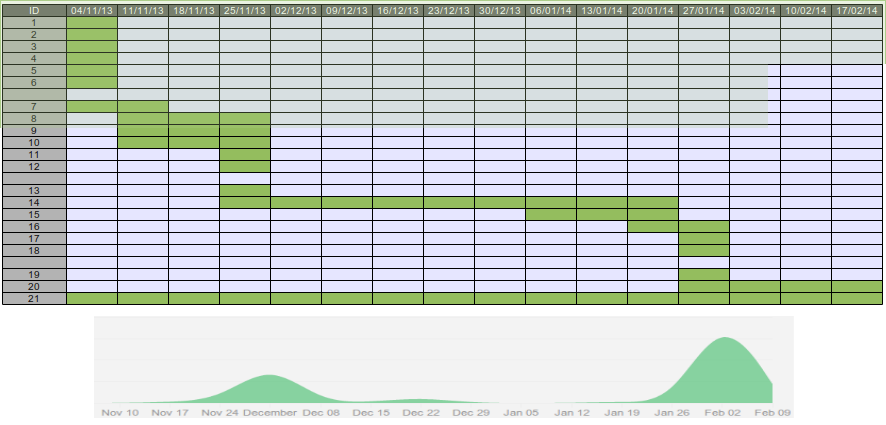
\includegraphics[scale=0.48]{images/GanttChart.png}

\begin{table}[H]
\centering
\begin{tabular}{|p{1.2cm}|p{8cm}|p{5cm}|}

\end{tabular}
\end{table}


% TODO:
% -> highlight changes in risk register and development plan - needs to be "appropriately reviewed and revised when necessary"
% -> evidence that the risks have been considered in the planning of the development

\section{Risk register}
\label{sec:riskregister}

A risk assessment has been performed as part of the interim
report to ensure the team is aware of any problems which could later
arise, and to provide a guide as to how to react when such problems
occur. The hazards (risks) have been identified by examining the 
current literature \cite{boehm1991software,jones1998minimizing}, drawing upon team members' past experiences and group 
discussion. Classification of the identified hazards, their impact on the system and their probability of occurrence is performed 
in accordance with the Risk Management Guide for Information Technology 
Systems \cite{stoneburner2002risk}. The areas these hazards impact were then analysed, as 
well as the probability of occurrence. These are then weighted so 
that we can identify the risks which are likely to 
have the greatest detrimental effect on the project. The likelihood 
score (LS), impact score (IS) and risk matrix score (RS) are listed 
in the table below.

\begin{longtable}[H]{| p{0.65cm} | p{2cm} | p{0.3cm} | p{0.3cm} | p{2.4cm} | p{3cm} | p{2.7cm} | p{0.4cm} |}
  \hline
  \cellcolor{titleColor}\textbf{Risk ID} &
  \cellcolor{titleColor}\textbf{Risk} &
  \cellcolor{titleColor}\textbf{LS} &
  \cellcolor{titleColor}\textbf{IS} &
  \cellcolor{titleColor}\textbf{Impact Description} &
  \cellcolor{titleColor}\textbf{Mitigation} &
  \cellcolor{titleColor}\textbf{Contingency} &
  \cellcolor{titleColor}\textbf{RS}\\
  
  \hline \textbf{R.1}
  & Loss of team member(s)
  & 6
  & 3
  & Internal and/or deadline failure
  & Ensure that no work relating to the project is outside of team
  version control; use of scrum methodology proactively aids work
  reallocation, ensuring team members are aware of all assigned work
  & Reallocation of work across remaining team members, may have to notify customer and possible deadline extension
  & 18 \\
  
  \hline \textbf{R.2}
  & Personnel under performance
  & 6
  & 3
  & Internal and/or deadline failure
  & Team strengths and weaknesses identified and work assigned appropriately, slack built into the schedule to account for under performance
  & Reallocation of work across remaining team members, may have to notify customer and possible deadline extension
  & 18 \\
  
  \hline \textbf{R.3}
  & Time pressures limiting amount of development time
  & 
  & 
  & Missing deadline, not fulfilling requirements, low quality deliverables
  & Define scope of work early, commit to complete requirements and allocate work to sprints 
  & Reduce functionality required and/or notify customer of later delivery
  & \\
  
  \hline \textbf{R.4}
  & Developing user interface that does not satisfy users requirements
  & 
  & 
  & Poor user experience, loss of confidence in the solution
  & Continuous, iterative development process, regularly incorporating users feedback on interface
  & Redevelop user interface
  & \\
  
  \hline \textbf{R.5}
  & Adding more functionality than necessary
  & 
  & 
  & Additional, unnecessary functionality, possible deadline miss
  & Ensure a clear, shared vision of the prototype system and collective ownership with open communication
  & \hl{???}
  & \\
  
  \hline \textbf{R.6}
  & Deprecation of required Google App Engine functionality
  & 
  & 
  & Unable to deliver required functionality
  & Research pending deprecations to ensure required functionality will be supported
  & Move to another key-store database (relatively simple)
  & \\
  
  
  \hline \textbf{R.7}
  & Communic-ations link to Google App Engine fails
  & 
  & 
  & Loss of service to users, loss of confidence in the system
  & A final commercial version would use the premium Google service which guarantees an uptime of at least 99.95\% (\nfrit10)
  & Additional data abstraction layer could be built to interface with another database service
  & \\
  
  \hline \textbf{R.8}
  & Data interception between our application and Google App Engine 
  & 
  & 
  & Loss of confidence in the system
  & A final system would encrypt traffic between our system and Google App Engine, currently just sending (non-sensitive) test data
  & Additional penetration testing to identify security flaws
  & \\
  
  \hline \textbf{R.9}
  & Data write/read times to/from Google App Engine too slow
  & 
  & 
  & Create a task backlog: gradual increase in load until system
  is non-operational (failure to meet capacity requirement \nfrit9)
  & Load testing of system throughout development to ensure \nfrit9
  & Re-engineering of system, possible need to switch datastore
  & \\
  
  \hline \textbf{R.10}
  & Implemen-tation does not facilitate data storage for a variety of systems
  & 
  & 
  & Failure to meet key modifiability requirements 
  & Adoption of a key-value database allows us the flexibility to store a variety of data
  & Examination of data we are struggling to store and implementation of additional data gateway for it
  & \\  
  
  \hline \textbf{R.11}
  & System performance required unattainable
  & 2
  & 4
  & \hl{Could cause }
  & Choice of implementation or choice of utilised hardware must offer
  enough in the way of performance to facilitate acceptable system
  performance.
  & All of, or combination of: optimisation of code, use of faster
  hardware, use of faster networks
  & 8 \\    
  
  \hline \textbf{R.12}
  & Included analysis components computing incorrect values
  & 
  & 
  & Failing to meet fundamental requirements, customer loses confidence in the system
  & Adopting a test driven approach to development throughout the development process
  & Re-engineering of failing components
  & \\
  
  \hline \textbf{R.13}
  & Analysis component computation too slow
  & 
  & 
  & Creates an analysis task backlog: gradual increase in load until system
  is non-operational
  & Load testing of analysis component throughout development, code optimisations 
  & Re-engineering of analysis components
  & \\  
  
  \hline \textbf{R.14}
  & Notification computation too slow
  & 
  & 
  & Creates a notification backlog: gradual increase in load until system
  is non-operational
  & Load testing of notification component throughout development, code optimisations 
  & Re-engineering of notification system
  & \\
  
  \hline \textbf{R.15}
  & GitHub becomes unavailable for a prolonged period of time
  & 
  & 
  & Difficulty merging work from different developers' machines
  & Distributed nature of Git means little work would be lost
  & Host our own git server within the Computer Science Department
  & \\ 
  
  \hline \textbf{R.16}
  & Malicious destruction of code repository on GitHub
  & 
  & 
  & \hl{???}
  & Two-step authentication used on GitHub, distributed nature of Git means little work would be lost
  & Host our own git server within the Computer Science Department
  & \\    
    
  \hline
\end{longtable}       

The likelihood score defines probability of something occurring. Utilising
\textit{Kents Words of Estimative Probability}\cite{kent1966strategic}, with
`certain' weighted $7$ and `impossible' weighted $1$.

\begin{longtable}[H]{|c|c|l|c|c|c|c|c|}
  \cline{4-8} \multicolumn{3}{c|}{} & \multicolumn{5}{ c| }{Impact Score (Least$\rightarrow$Most)} \\
  \cline{4-8} \multicolumn{3}{c|}{} & 1 & 2 & 3 & 4 & 5 \\
  \cline{4-8} \multicolumn{3}{c|}{} & Negligible& Minor & Moderate& Major & Catastrophic \\

  \hline \multirow{7}{*}{Likelihood Score} & 7 & Certain & 7 & 14 & 21 & 28 & 35 \\

  \cline{2-8} & 6 & Almost certain & 6 & 12 & 18 & 24 & 30 \\
  \cline{2-8} & 5 & Probable& 5 & 10 & 15 & 20 & 25 \\
  \cline{2-8} & 4 & Chances about even & 4 & 8 & 12 & 16 & 20 \\
  \cline{2-8} & 3 & Probably not & 3 & 6 & 9 & 12 & 15 \\
  \cline{2-8} & 2 & Almost certainly not & 2 & 4 & 6 & 8 & 10 \\
  \cline{2-8} & 1 & Impossible & 1 & 2 & 3 & 4 & 5 \\
  \hline
\end{longtable}

\begin{longtable}[H]{ | p{2cm} | p{4cm} | p{8.5cm} | }
  \hline
  \cellcolor{titleColor}\textbf{Score} &
  \cellcolor{titleColor}\textbf{Risk Level} &
  \cellcolor{titleColor}\textbf{Recommended Response} \\

  \hline \textbf{23-35} & HIGH & Mitigation plan is
  required. Immediate action is required.\\

  \hline \textbf{11-22} & MEDIUM & To be included in the action plan
  and reviewed.\\

  \hline \textbf{0-10}& LOW & Included in action plan in limited
  scope. Minimum review. \\
  \hline
\end{longtable}

\section{Customer communication}
\label{sec:communication}

Our initial communication with the customer for this stage of the project was in the form of a face to face meeting where we received feedback on our previous report. This feedback was recorded and acted upon, including extending the risk register to include more technical risks and examining the qualities of the system. Our next contact was through email in which we sent a low fidelity prototype of the HUMS admin centre, explaining our idea of hosting a HUMS as a SaaS or PaaS, to which the customer replied the idea was interesting and suggested some small improvements. 

After each communication with the customer we organised group meetings within two days to discuss the feedback issued and to collaborate on any improvements to our solution we could make based upon the feedback. In our next face to face meeting with the customer we explained our architectural ideas and discussed the test application, we then went on to have a team meeting where we planned how to monitor the test application. We then sent the customer a series of emails detailing implementation and architectural decisions, including the qualities and views we identified, and also an example of a reporting engine. The customer replied with helpful feedback including additional qualities they felt were important to the system and positive feedback on the module view diagram.


\vfill
\bibliography{report-refs}
\bibliographystyle{IEEEtran}
\end{document}
